\documentclass[../../Thesis.tex]{subfiles}

\newcommand\MyBox[2]{
  \fbox{\lower0.75cm
    \vbox to 1.7cm{\vfil
      \hbox to 1.7cm{\hfil\parbox{1.4cm}{#1\\#2}\hfil}
      \vfil}%
  }%
}

% “  ”

\begin{document}
	In this chapter, we will analyze the experiment we have made and discuss the measurements we have collected. The experiments will be analyzed from three different perspectives: feature analysis, performance metrics, and model performances. At the beginning we will analyze the feature time series values of nominal robots against faulty robots, we will then proceed on explaining which metrics we have used to judge the model performances, and, in the end, we will evaluate the model performances themselves.
	
	\section{Data Sets Analysis}
		In this section we will graphically show the values assumed by each feature and if they present some distinguishing characteristics between nominal and faulty agents. 
		\subsection{Flocking Features Analysis}
		\label{sec:Experiments:flocking_feature_analysis}
			The flocking task is explained in Section \ref{sec:Flocking}. The robot trajectories can be seen in Figure \ref{fig:ARGoS_flocking_trajectories}. From now on, we will analyze the features explained in Section \ref{sec:feature_computation}. The direction feature will not be analyzed since it is unfeasible to show it graphically and useless to numerically analyze it. In this example, we will analyze a simulation of 15 agents with 1 faulty agent. In this section, we will analyze a flocking task starting from the East position. The fault is injected at 150 $s$ and the robot rotates around a fixed point until the end of the simulation. For each second we have 10 timesteps.
			
			\subsubsection{Speed}
				The speed feature is one of the most characteristics since all of our faults influence this measure. It is possible to immediately distinguish the faulty robot behavior from the nominal robots. In the graphs in Figure \ref{fig:flocking_speed} we can see that the faulty robot does not change speed after the fault is injected. 
				\begin{figure}
					\centering
					\subfloat[Flocking nominal agents speed feature values.
						\label{fig:flocking_nominal_speed_feature}]{
						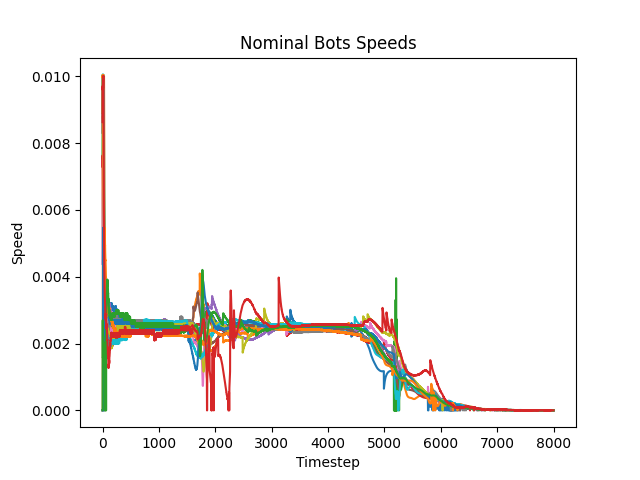
\includegraphics[scale=0.4]{../../Images/Experiments/flocking_15_East_6_percent_rotating_fault_after_1500_gain_1000/Nominal_Bots_Speeds.png}
					}
					\quad
					\subfloat[Flocking faulty agents speed feature values.\label{fig:flocking_faulty_speed_feature}]{
						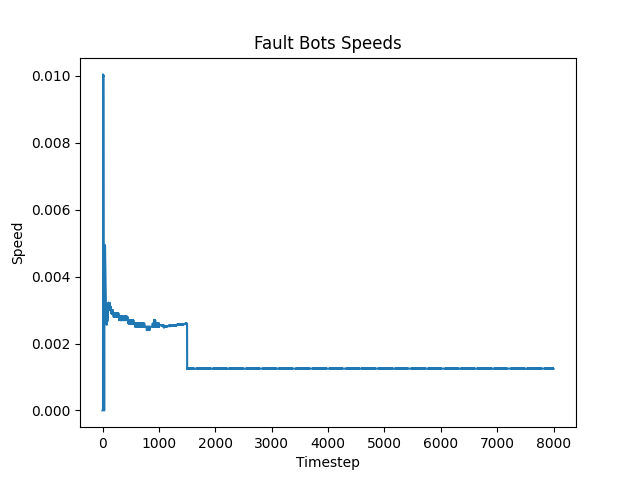
\includegraphics[scale=0.4]{../../Images/Experiments/flocking_15_East_6_percent_rotating_fault_after_1500_gain_1000/Fault_Bots_Speeds.png}
					}
					\caption{Flocking speed feature values.}
					\label{fig:flocking_speed}
				\end{figure}
			
			\subsubsection{Cumulative Speed}
				The cumulative speed feature (Figure \ref{fig:flocking_cumulative_speed}) is a rounded version of the speed feature that holds some information about the timestep in the \verb|time-window|. This feature has identical characteristics to the speed feature and it is possible to distinguish the faulty robot at first sight. The \verb|time-window| parameter is set to $10$ and the values of the feature show the correlation between the two features.
				\begin{figure}
					\centering
					\subfloat[Flocking nominal agents cumulative speed feature values.
						\label{fig:flocking_nominal_cumulative_speed_feature}]{
						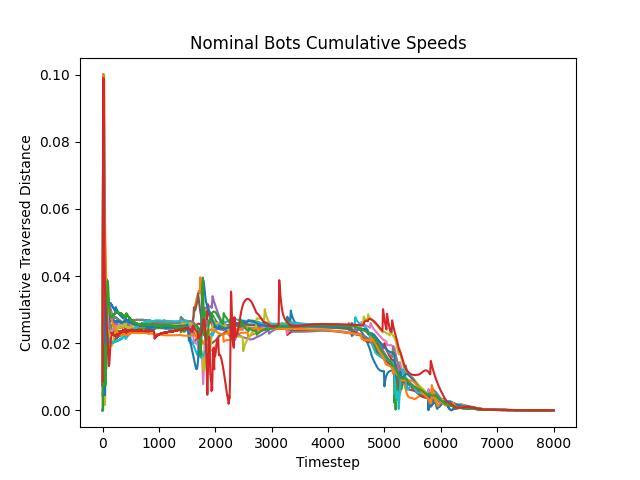
\includegraphics[scale=0.4]{../../Images/Experiments/flocking_15_East_6_percent_rotating_fault_after_1500_gain_1000/Nominal_Bots_Cumulative_Speeds.png}
					}
					\quad
					\subfloat[Flocking faulty agents cumulative speed feature values.\label{fig:flocking_faulty_cumulative_speed_feature}]{
						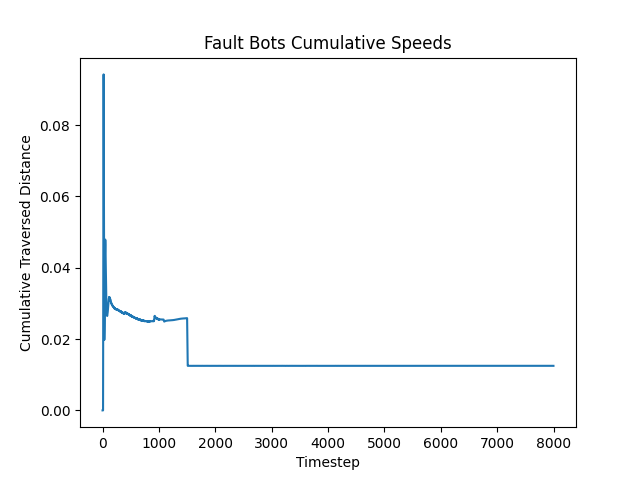
\includegraphics[scale=0.4]{../../Images/Experiments/flocking_15_East_6_percent_rotating_fault_after_1500_gain_1000/Fault_Bots_Cumulative_Speeds.png}
					}
					\caption{Flocking cumulative speed feature values.}
					\label{fig:flocking_cumulative_speed}
				\end{figure}
			
			\subsubsection{Neighbors Number}
				The neighbors number feature is very interesting for the flocking task since the agents have to keep a formation at a certain distance from one another. In Figure \ref{fig:flocking_neighbors_number} we can see that the faulty agent has a high number of neighbors at the start of the simulation, however, soon after the fault is injected, this value drastically drops denoting a separation of the agent from the swarm. \\
				In this situation the neighborhood radius value has been set to 2 $m$. This value has to be fine tuned in order to have significant results.
				\begin{figure}
					\centering
					\subfloat[Flocking nominal agents neighbors number feature values.
						\label{fig:flocking_nominal_neighbors_number_feature}]{
						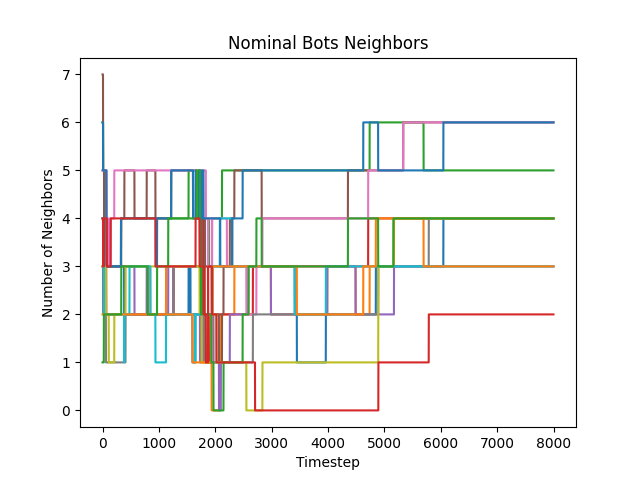
\includegraphics[scale=0.4]{../../Images/Experiments/flocking_15_East_6_percent_rotating_fault_after_1500_gain_1000/Nominal_Bots_Neighbors.png}
					}
					\quad
					\subfloat[Flocking faulty agents neighbors number feature values.\label{fig:flocking_faulty_neighbors_number_feature}]{
						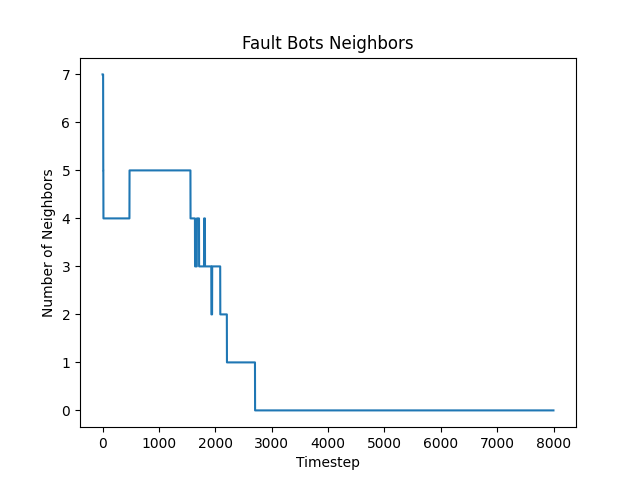
\includegraphics[scale=0.4]{../../Images/Experiments/flocking_15_East_6_percent_rotating_fault_after_1500_gain_1000/Fault_Bots_Neighbors.png}
					}
					\caption{Flocking neighbors number feature values.}
					\label{fig:flocking_neighbors_number}
				\end{figure}
			
			\subsubsection{Neighbors Average Distance}
				The neighbors average distance feature highlights information similar to the neighbors number feature with opposite values, in this situation, the high value of the feature denotes a separation of the agent from the swarm. This feature is interesting for the flocking task, as the neighbors number feature, because it describes the behavior of the agent with respect to the other agents.  In Figure \ref{fig:flocking_neighbors_average_distance} we can see that the faulty agent detaches from the swarm after the fault is injected.
				\begin{figure}
					\centering
					\subfloat[Flocking nominal agents neighbors average distance feature values.
						\label{fig:flocking_nominal_neighbors_average_distance_feature}]{
						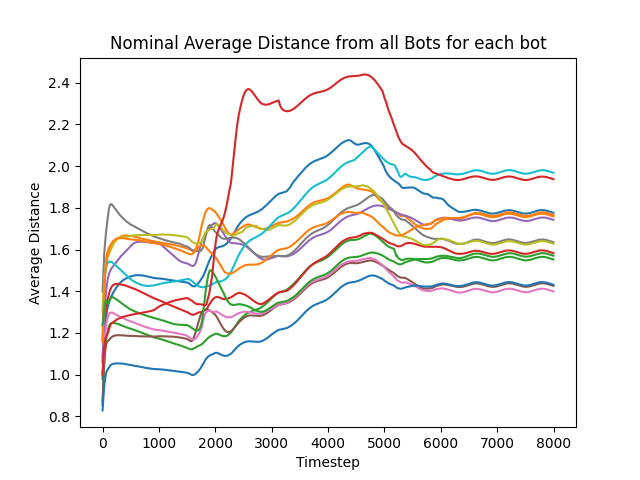
\includegraphics[scale=0.4]{../../Images/Experiments/flocking_15_East_6_percent_rotating_fault_after_1500_gain_1000/Nominal_Average_Distance_from_all_Bots_for_each_bot.png}
					}
					\quad
					\subfloat[Flocking faulty agents neighbors average distance feature values.\label{fig:flocking_faulty_neighbors_average_distance_feature}]{
						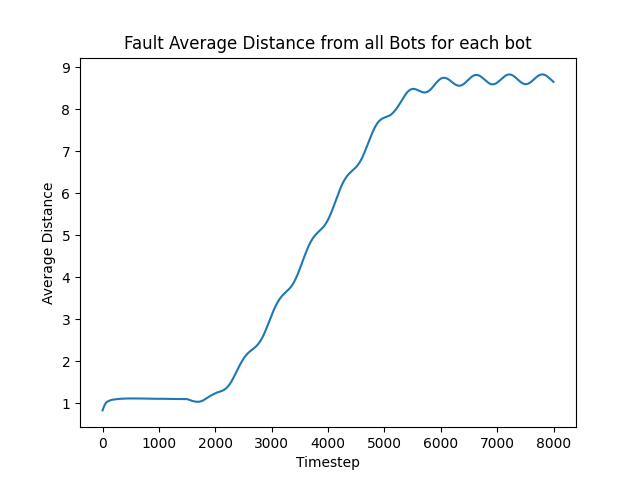
\includegraphics[scale=0.4]{../../Images/Experiments/flocking_15_East_6_percent_rotating_fault_after_1500_gain_1000/Fault_Average_Distance_from_all_Bots_for_each_bot.png}
					}
					\caption{Flocking neighbors average distance feature values.}
					\label{fig:flocking_neighbors_average_distance}
				\end{figure}
			
			\subsubsection{Centroid Distance}
				The centroid distance feature is a simplified version of the neighbors average distance feature since it is easier to compute. From the graphs in Figure \ref{fig:flocking_centroid_distance} we can see that the values have a similar shape to the values shown in Figure \ref{fig:flocking_neighbors_average_distance} and show similar values, this is because the distance from the centroid can be seen as a mean value of the distance from the other agents.
				\begin{figure}
					\centering
					\subfloat[Flocking nominal agents centroid distance feature values.
						\label{fig:flocking_nominal_centroid_distance_feature}]{
						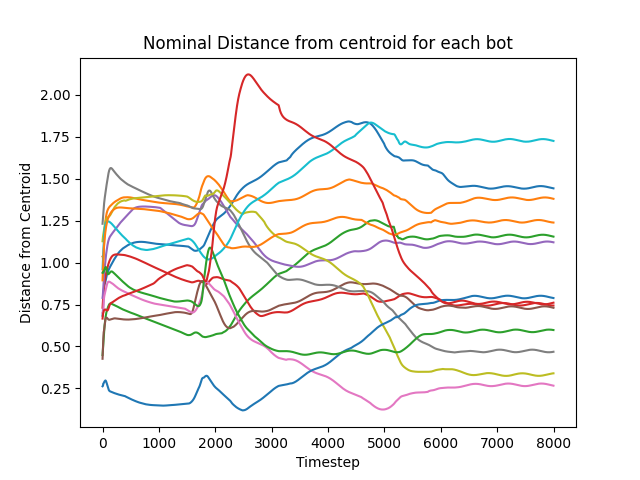
\includegraphics[scale=0.4]{../../Images/Experiments/flocking_15_East_6_percent_rotating_fault_after_1500_gain_1000/Nominal_Distance_from_centroid_for_each_bot.png}
					}
					\quad
					\subfloat[Flocking faulty agents centroid distance feature values.\label{fig:flocking_faulty_centroid_distance_feature}]{
						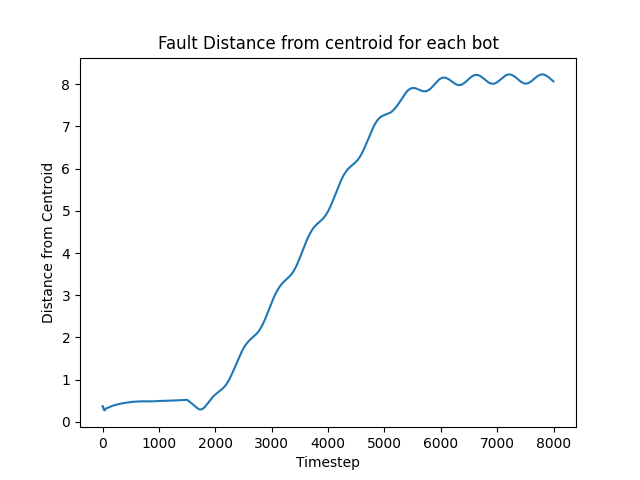
\includegraphics[scale=0.4]{../../Images/Experiments/flocking_15_East_6_percent_rotating_fault_after_1500_gain_1000/Fault_Distance_from_centroid_for_each_bot.png}
					}
					\caption{Flocking centroid distance feature values.}
					\label{fig:flocking_centroid_distance}
				\end{figure}
			
			\subsubsection{Cumulative Centroid Distance}
				The cumulative centroid distance feature is a feature that holds some information about the past values. The concept behind this feature is similar to the one of the cumulative speed feature. Since this feature is a sum of the past values of the centroid distance feature, these two feature show high correlation and the values in the Figure \ref{fig:flocking_cumulative_centroid_distance} depicts the values of Figure \ref{fig:flocking_centroid_distance} multiplied by the \verb|time-window| parameter.
				\begin{figure}
					\centering
					\subfloat[Flocking nominal agents centroid distance feature values.
						\label{fig:flocking_nominal_cumulative_centroid_distance_feature}]{
						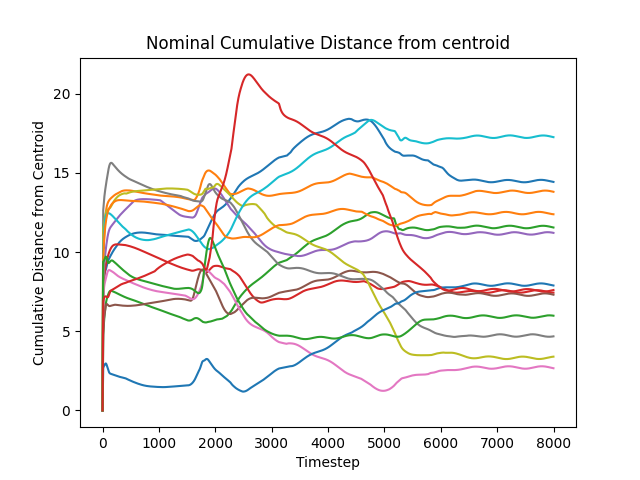
\includegraphics[scale=0.4]{../../Images/Experiments/flocking_15_East_6_percent_rotating_fault_after_1500_gain_1000/Nominal_Cumulative_Distance_from_centroid.png}
					}
					\quad
					\subfloat[Flocking faulty agents centroid distance feature values.\label{fig:flocking_faulty_cumulative_centroid_distance_feature}]{
						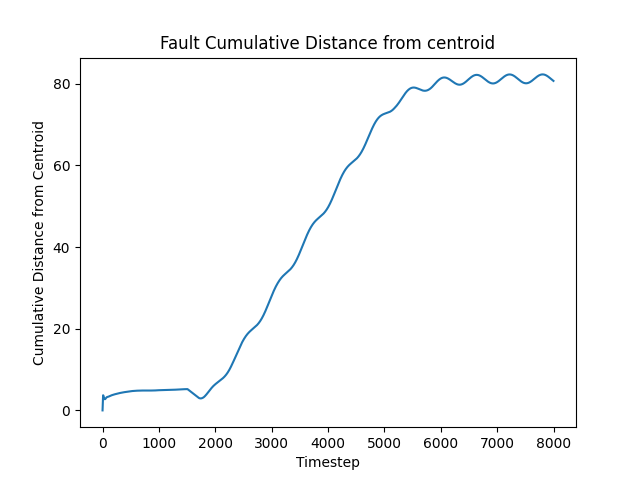
\includegraphics[scale=0.4]{../../Images/Experiments/flocking_15_East_6_percent_rotating_fault_after_1500_gain_1000/Fault_Cumulative_Distance_from_centroid.png}
					}
					\caption{Flocking centroid distance feature values.}
					\label{fig:flocking_cumulative_centroid_distance}
				\end{figure}
				
			\subsubsection{Position Entropy}
				The position entropy feature aims at identifying how many different positions are covered by the agent in the last \verb|time-window| timesteps. The graphs shown in Figure \ref{fig:flocking_position_entropy} do not show any interesting information about the task execution since the faulty agent doesn't have different values than nominal agents. Like we said for the \verb|neighborhood-radius| parameter, the \verb|time-window| parameter has to be fine tuned for each different task such that the position entropy feature shows interesting values.
				\begin{figure}
					\centering
					\subfloat[Flocking nominal agents position entropy feature values.
						\label{fig:flocking_nominal_position_entropy_feature}]{
						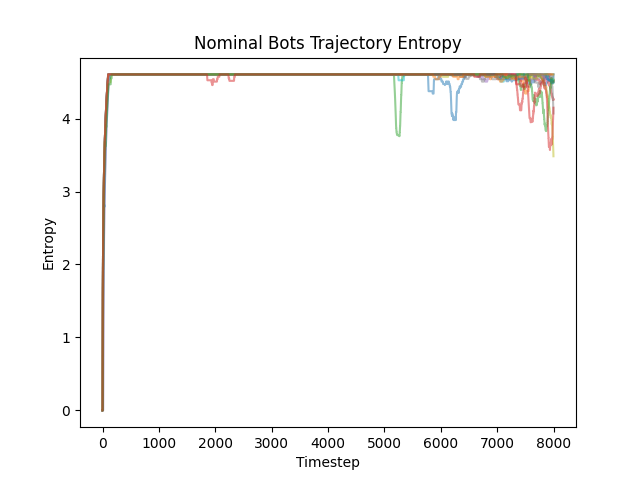
\includegraphics[scale=0.4]{../../Images/Experiments/flocking_15_East_6_percent_rotating_fault_after_1500_gain_1000/Nominal_Bots_Trajectory_Entropy.png}
					}
					\quad
					\subfloat[Flocking faulty agents position entropy feature values.\label{fig:flocking_faulty_position_entropy_feature}]{
						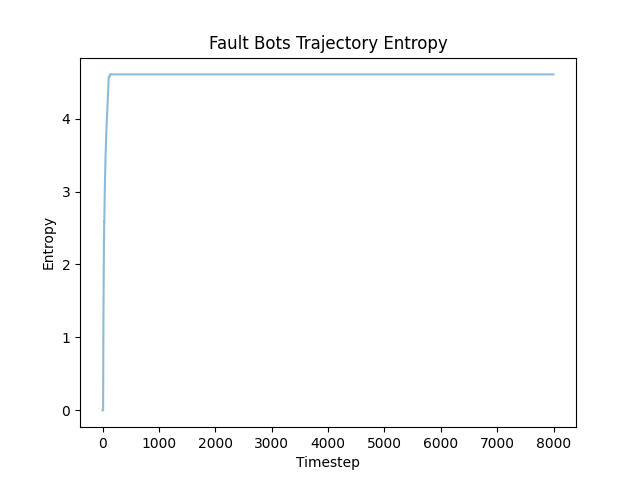
\includegraphics[scale=0.4]{../../Images/Experiments/flocking_15_East_6_percent_rotating_fault_after_1500_gain_1000/Fault_Bots_Trajectory_Entropy.png}
					}
					\caption{Flocking position entropy feature values.}
					\label{fig:flocking_position_entropy}
				\end{figure}
			
			\subsubsection{Area Coverage}
			\label{sec:flocking_area_coverage} %
				The area coverage feature is divided into 4 different time series. The time series shown in Figure \ref{fig:flocking_nominal_agents_area_coverage} depict the values assumed by the area coverage feature of the nominal agents with different levels of area partitioning. From the left, we can see the values in the case of 4 subdivisions, 16 subdivisions, 64 subdivisions, and then 256 subdivisions. We can see that the maximum value reached by the feature decreases with the increase of the area subdivisions, this is because, with the increase of the definition in area partitioning, some areas are too small to be covered by any agent.\\
				The time series shown in Figure \ref{fig:flocking_faulty agents_area_coverage} depict the values assumed by the area coverage feature of the faulty agents.  The graphs are organized like in Figure \ref{fig:flocking_nominal_agents_area_coverage}. The most important difference between nominal and faulty agents is that the faulty agent feature usually reaches lower values than the nominal agents.
				\begin{figure}[H]
					\centering
					\subfloat[4 subdivisions.
						\label{fig:flocking_nominal_4_subdivisions_area_coverage_feature}]{
						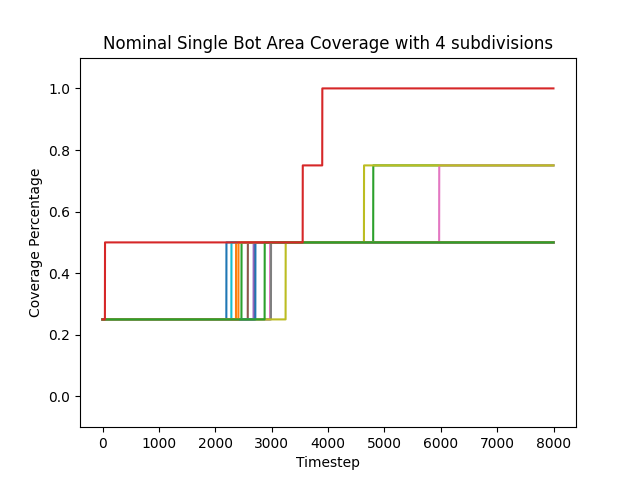
\includegraphics[scale=0.22]{../../Images/Experiments/flocking_15_East_6_percent_rotating_fault_after_1500_gain_1000/Nominal_Single_Bot_Area_Coverage_with_4_subdivisions.png}
					}
					\thinspace
					\subfloat[16 subdivisions.
						\label{fig:flocking_nominal_16_subdivisions_area_coverage_feature}]{
						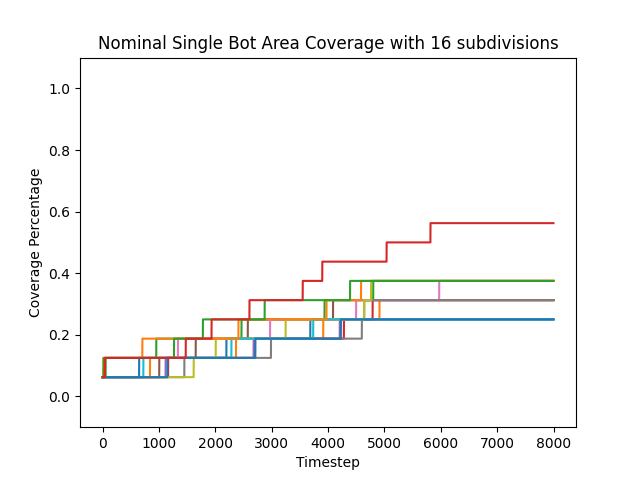
\includegraphics[scale=0.22]{../../Images/Experiments/flocking_15_East_6_percent_rotating_fault_after_1500_gain_1000/Nominal_Single_Bot_Area_Coverage_with_16_subdivisions.png}
					}
					\thinspace
					\subfloat[64 subdivisions.
						\label{fig:flocking_nominal_64_subdivisions_area_coverage_feature}]{
						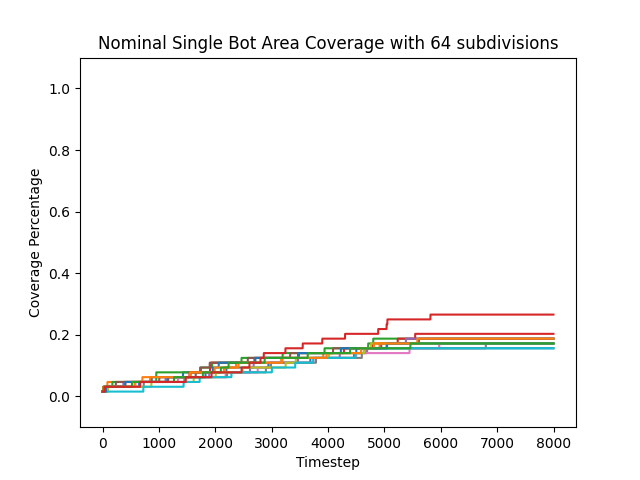
\includegraphics[scale=0.22]{../../Images/Experiments/flocking_15_East_6_percent_rotating_fault_after_1500_gain_1000/Nominal_Single_Bot_Area_Coverage_with_64_subdivisions.png}
					}
					\thinspace
					\subfloat[256 subdivisions.
						\label{fig:flocking_nominal_256_subdivisions_area_coverage_feature}]{
						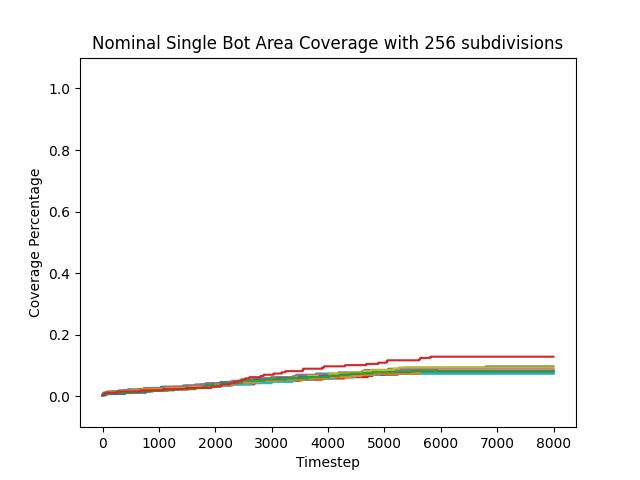
\includegraphics[scale=0.22]{../../Images/Experiments/flocking_15_East_6_percent_rotating_fault_after_1500_gain_1000/Nominal_Single_Bot_Area_Coverage_with_256_subdivisions.png}
					}
					\caption{Flocking nominal agents area coverage feature values.}
					\label{fig:flocking_nominal_agents_area_coverage}
				\end{figure}
			
				\begin{figure}[H]
					\centering
					\subfloat[4 subdivisions.\label{fig:flocking_faulty_4_subdivisions_area_coverage_feature}]{
						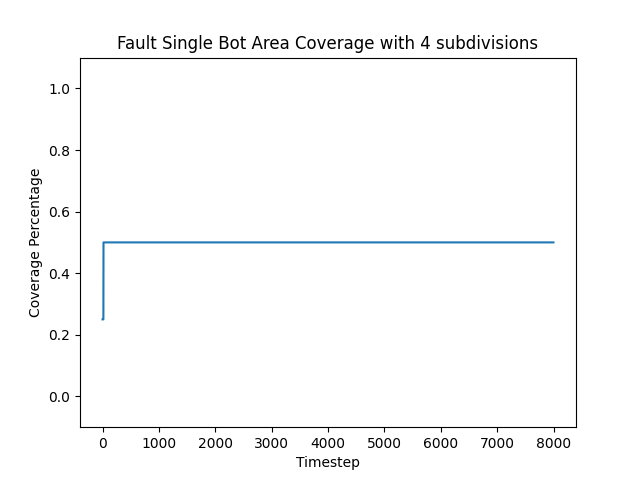
\includegraphics[scale=0.22]{../../Images/Experiments/flocking_15_East_6_percent_rotating_fault_after_1500_gain_1000/Fault_Single_Bot_Area_Coverage_with_4_subdivisions.png}
					}
					\subfloat[16 subdivisions.\label{fig:flocking_faulty_16_subdivisions_area_coverage_feature}]{
						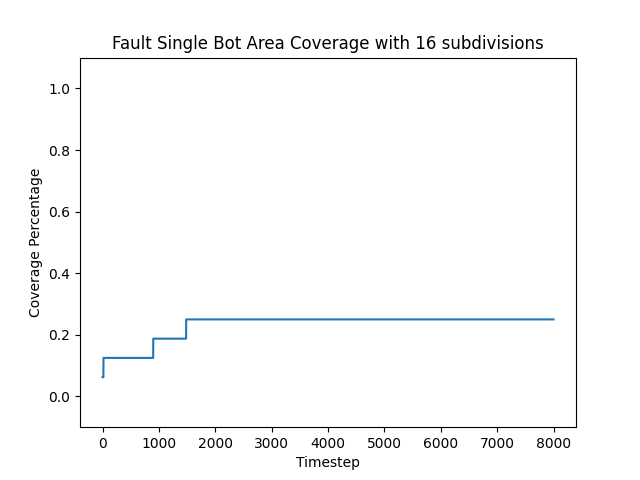
\includegraphics[scale=0.22]{../../Images/Experiments/flocking_15_East_6_percent_rotating_fault_after_1500_gain_1000/Fault_Single_Bot_Area_Coverage_with_16_subdivisions.png}
					}
					\subfloat[64 subdivisions.\label{fig:flocking_faulty_64_subdivisions_area_coverage_feature}]{
						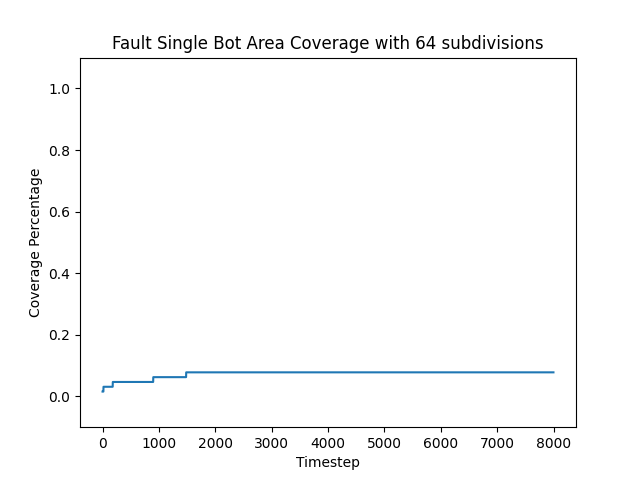
\includegraphics[scale=0.22]{../../Images/Experiments/flocking_15_East_6_percent_rotating_fault_after_1500_gain_1000/Fault_Single_Bot_Area_Coverage_with_64_subdivisions.png}
					}
					\subfloat[256 subdivisions.\label{fig:flocking_faulty_256_subdivisions_area_coverage_feature}]{
						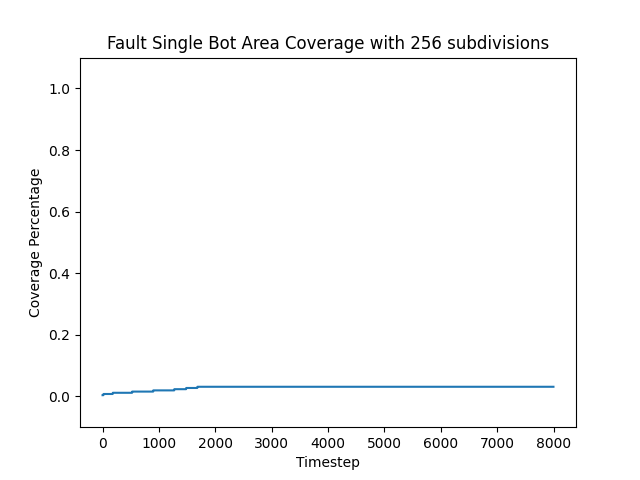
\includegraphics[scale=0.22]{../../Images/Experiments/flocking_15_East_6_percent_rotating_fault_after_1500_gain_1000/Fault_Single_Bot_Area_Coverage_with_256_subdivisions.png}
					}
					\caption{Flocking faulty agents area coverage feature values.}
					\label{fig:flocking_faulty agents_area_coverage}
				\end{figure}
					
			\subsubsection{Area Coverage Speed}
				The area coverage speed feature holds information about the value increments of the area coverage feature. The graphs are organized like the ones of the area coverage feature. The most distinguishing aspect of this feature is that we can observe the faulty robot that stops exploring earlier than the nominal agents due to the injection of the fault.
				\begin{figure}[H]
					\centering
					\subfloat[4 subdivisions.
						\label{fig:flocking_nominal_4_subdivisions_area_coverage_speed_feature}]{
						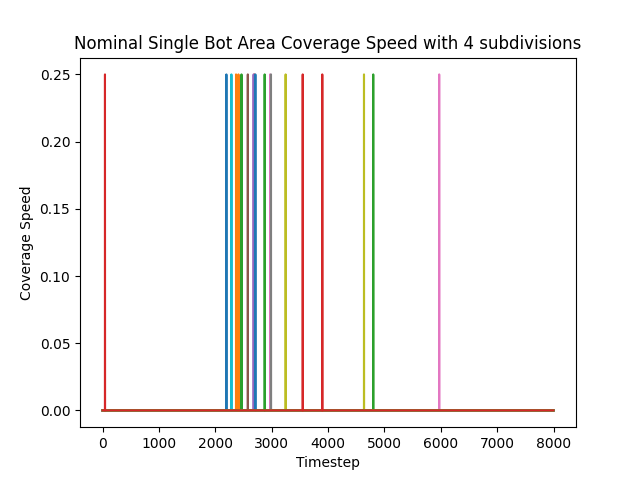
\includegraphics[scale=0.22]{../../Images/Experiments/flocking_15_East_6_percent_rotating_fault_after_1500_gain_1000/Nominal_Single_Bot_Area_Coverage_Speed_with_4_subdivisions.png}
					}
					\thinspace
					\subfloat[16 subdivisions.
						\label{fig:flocking_nominal_16_subdivisions_area_coverage_speed_feature}]{
						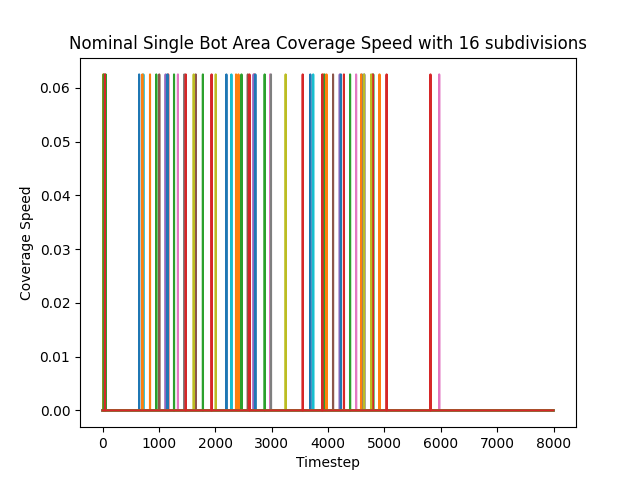
\includegraphics[scale=0.22]{../../Images/Experiments/flocking_15_East_6_percent_rotating_fault_after_1500_gain_1000/Nominal_Single_Bot_Area_Coverage_Speed_with_16_subdivisions.png}
					}
					\thinspace
					\subfloat[64 subdivisions.
						\label{fig:flocking_nominal_64_subdivisions_area_coverage_speed_feature}]{
						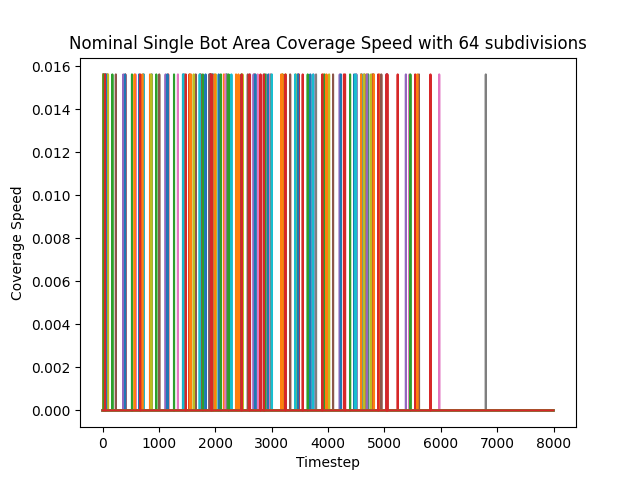
\includegraphics[scale=0.22]{../../Images/Experiments/flocking_15_East_6_percent_rotating_fault_after_1500_gain_1000/Nominal_Single_Bot_Area_Coverage_Speed_with_64_subdivisions.png}
					}
					\thinspace
					\subfloat[256 subdivisions.
						\label{fig:flocking_nominal_256_subdivisions_area_coverage_speed_feature}]{
						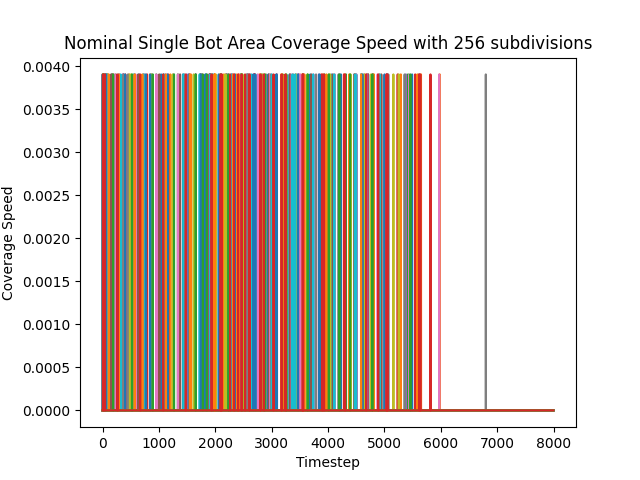
\includegraphics[scale=0.22]{../../Images/Experiments/flocking_15_East_6_percent_rotating_fault_after_1500_gain_1000/Nominal_Single_Bot_Area_Coverage_Speed_with_256_subdivisions.png}
					}
					\caption{Flocking nominal agents area coverage speed feature values.}
					\label{fig:flocking_nominal_agents_area_coverage_speed_feature_values}
				\end{figure}
				
				\begin{figure}[H]
					\centering
					\subfloat[4 subdivisions.\label{fig:flocking_faulty_4_subdivisions_area_coverage_speed_feature}]{
						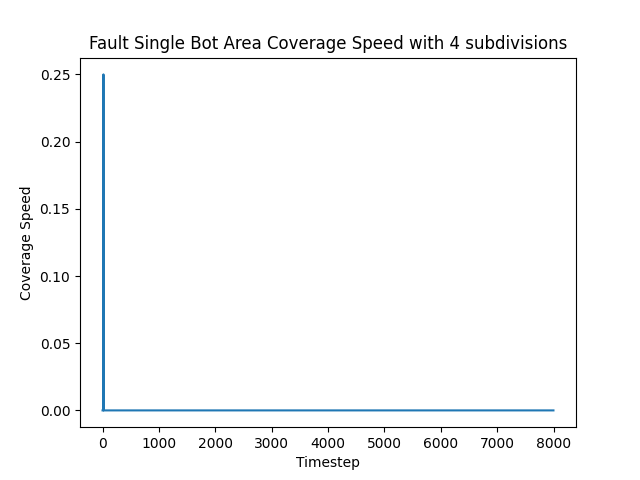
\includegraphics[scale=0.22]{../../Images/Experiments/flocking_15_East_6_percent_rotating_fault_after_1500_gain_1000/Fault_Single_Bot_Area_Coverage_Speed_with_4_subdivisions.png}
					}
					\thinspace
					\subfloat[16 subdivisions.\label{fig:flocking_faulty_16_subdivisions_area_coverage_speed_feature}]{
						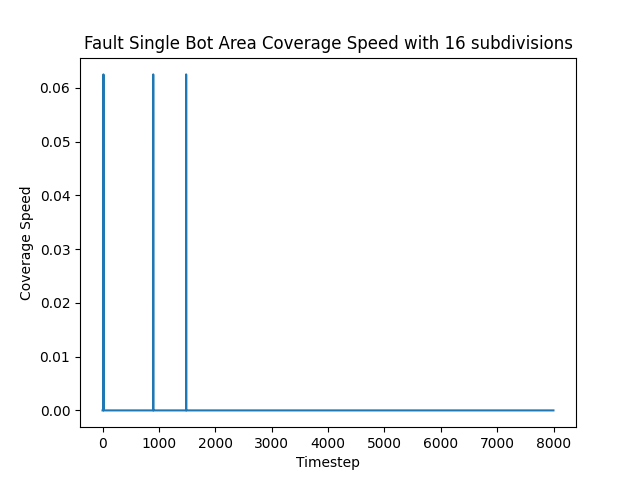
\includegraphics[scale=0.22]{../../Images/Experiments/flocking_15_East_6_percent_rotating_fault_after_1500_gain_1000/Fault_Single_Bot_Area_Coverage_Speed_with_16_subdivisions.png}
					}
					\thinspace
					\subfloat[64 subdivisions.\label{fig:flocking_faulty_64_subdivisions_area_coverage_speed_feature}]{
							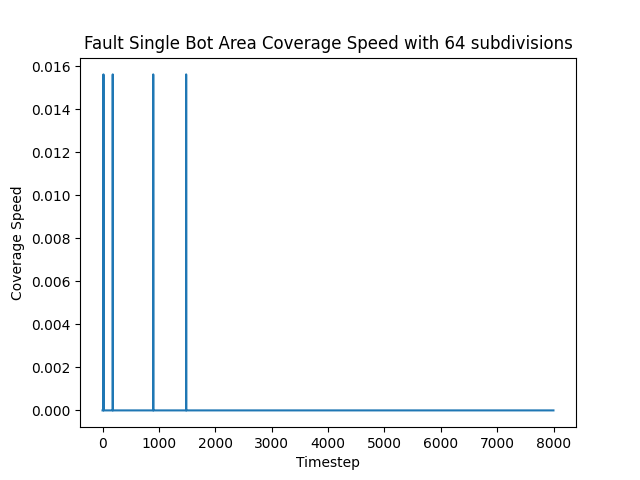
\includegraphics[scale=0.22]{../../Images/Experiments/flocking_15_East_6_percent_rotating_fault_after_1500_gain_1000/Fault_Single_Bot_Area_Coverage_Speed_with_64_subdivisions.png}
					}
					\thinspace
					\subfloat[256 subdivisions.\label{fig:flocking_faulty_256_subdivisions_area_coverage_speed_feature}]{
							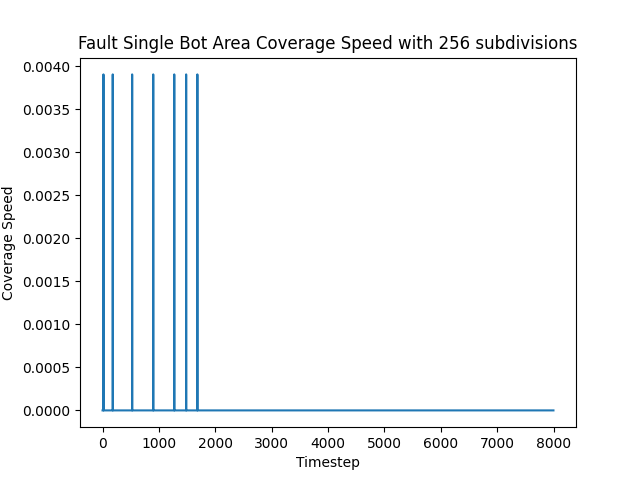
\includegraphics[scale=0.22]{../../Images/Experiments/flocking_15_East_6_percent_rotating_fault_after_1500_gain_1000/Fault_Single_Bot_Area_Coverage_Speed_with_256_subdivisions.png}
					}
					\caption{Flocking faulty agents area coverage speed feature values.}
					\label{fig:flocking_faulty_area_coverage_speed}
				\end{figure}
			
			\subsubsection{Global Features}
				The global features are those features that contain information about the overall behavior of the swarm in its entirety. These features should depict information about the execution of the task but do not contain information about the single agent, this characteristic is important because this kind of feature can not be considered fundamental for the objective of fault detection. The presence of these features is important whenever we use a model that can infer complex information from different features of the sample, i.e. convolutional neural networks.\\
				\textbf{Swarm Position} \\
				The swarm position feature is the coordinates of the centroid of the swarm. We can see the trajectory followed by the swarm centroid in Figure \ref{fig:flocking_swarm_trajectory} as the bright red line in the middle of the plot among nominal agents (Figure \ref{fig:flocking_nominal_swarm_trajectory}) and faulty agents (Figure \ref{fig:flocking_faulty_swarm_trajectory}).
					\begin{figure}
						\centering
						\subfloat[Swarm trajectory among nominal agents.
							\label{fig:flocking_nominal_swarm_trajectory}]{
							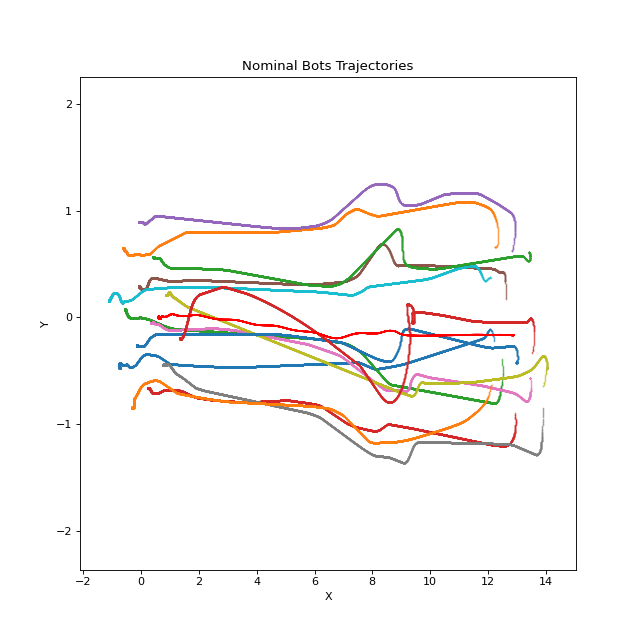
\includegraphics[scale=0.3]{../../Images/Experiments/flocking_15_East_6_percent_rotating_fault_after_1500_gain_1000/Nominal_Bots_Trajectories_with_swarm.png}
						}
						\quad
						\subfloat[Swarm trajectory among faulty agents.\label{fig:flocking_faulty_swarm_trajectory}]{
							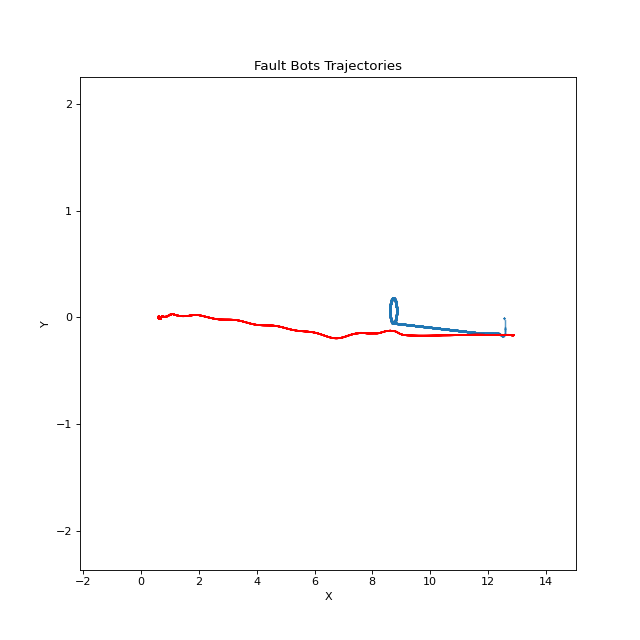
\includegraphics[scale=0.3]{../../Images/Experiments/flocking_15_East_6_percent_rotating_fault_after_1500_gain_1000/Fault_Bots_Trajectories_with_swarm.png}
						}
						\caption{Swarm trajectory.}
						\label{fig:flocking_swarm_trajectory}
					\end{figure}
					
					\textbf{Swarm Speed} \\
					The swarm speed feature represents the velocity of the swarm centroid. In Figure \ref{fig:flocking_swarm_speed}, we can see that the values have a high spike at the beginning when the robots move to get in flocking formation. The feature value stays constant until 1500 timesteps, namely 150 $s$, and then slowly drops to lower values after the fault is injected. This feature behavior perfectly mirrors the swarm centroid movement that is slowed down by the faulty agent.
					\begin{figure}
						\centering
						\includegraphics[scale=0.4]{../../Images/Experiments/flocking_15_East_6_percent_rotating_fault_after_1500_gain_1000/Swarm_speed.png}
						\caption{Swarm speed.}
						\label{fig:flocking_swarm_speed}
					\end{figure}
			\subsubsection{Swarm Area Coverage}
				The swarm area coverage features illustrate the percentage of area covered by the entirety of the swarm considered each agent. This feature is similar to the area coverage feature seen before in section Area Coverage. As stated above, this is a global feature and does not have the objective to directly identify the fault injection. Nonetheless, the graphs shown in Figure \ref{fig:flocking_swarm_area_coverage_feature_values} do not shown any sign of the presence of the fault injected after 150 $s$.
				\begin{figure}
					\centering
					\subfloat[Flocking swarm 4 subdivisions area coverage feature values.
						\label{fig:flocking_swarm_4_subdivisions_area_coverage_feature}]{
						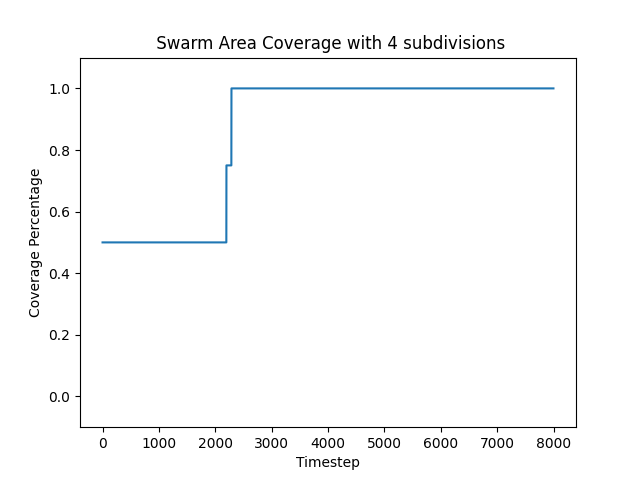
\includegraphics[scale=0.4]{../../Images/Experiments/flocking_15_East_6_percent_rotating_fault_after_1500_gain_1000/Swarm_Area_Coverage_with_4_subdivisions.png}
					}
					\quad
					\subfloat[Flocking swarm 16 subdivisions area coverage feature values.\label{fig:flocking_swarm_16_subdivisions_area_coverage_feature}]{
						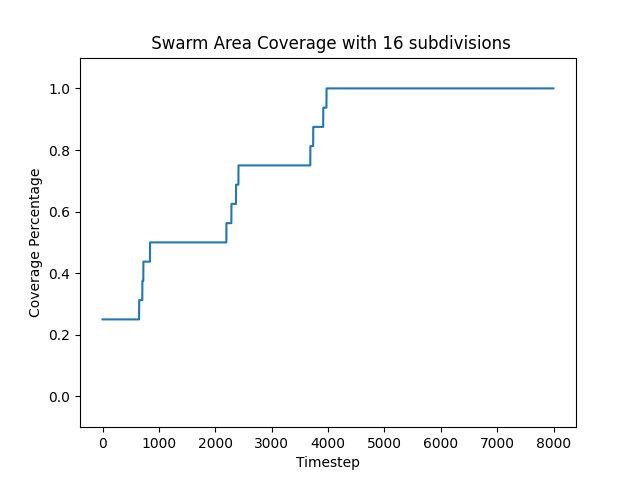
\includegraphics[scale=0.4]{../../Images/Experiments/flocking_15_East_6_percent_rotating_fault_after_1500_gain_1000/Swarm_Area_Coverage_with_16_subdivisions.png}
					}
					\quad
					\subfloat[Flocking swarm 64 subdivisions area coverage feature values.
						\label{fig:flocking_swarm_64_subdivisions_area_coverage_feature}]{
						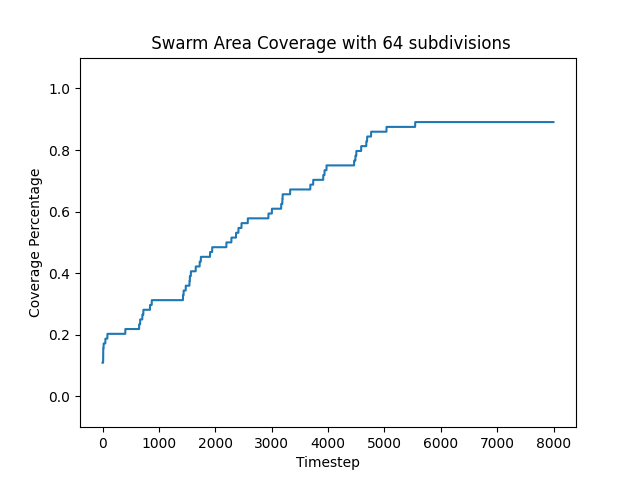
\includegraphics[scale=0.4]{../../Images/Experiments/flocking_15_East_6_percent_rotating_fault_after_1500_gain_1000/Swarm_Area_Coverage_with_64_subdivisions.png}
					}
					\quad
					\subfloat[Flocking swarm 256 subdivisions area coverage feature values.\label{fig:flocking_swarm_256_subdivisions_area_coverage_feature}]{
						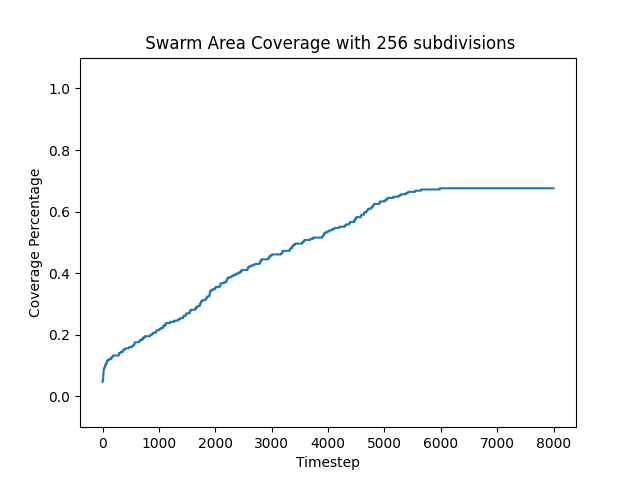
\includegraphics[scale=0.4]{../../Images/Experiments/flocking_15_East_6_percent_rotating_fault_after_1500_gain_1000/Swarm_Area_Coverage_with_256_subdivisions.png}
					}
					\caption{Flocking swarm area coverage feature values.}
					\label{fig:flocking_swarm_area_coverage_feature_values}
				\end{figure}
					
		\subsection{Foraging Features Analysis}
			The foraging task is explained in Section \ref{sec:Foraging}. The robot trajectories can be seen in Figure \ref{fig:ARGoS_foraging_trajectories}. In this example, we will analyze a simulation of 38 agents with 4 faulty agents. The fault is injected at 150 $s$ and the robots rotate around a fixed point until the end of the simulation. For each second we have 10 timesteps.
			\subsubsection{Speed}
				As stated for the flocking task, this feature is highly significant due to the nature of the faults injected. In Figure \ref{fig:foraging_speed} we can see that the faulty robots rotate do not reach high speeds after the fault is injected but their speed oscillates at values lower than the nominal agents. The oscillations of faulty agents' speed can be traced back to obstacle avoidance maneuvers or blockages in the nest area.
				\begin{figure}
					\centering
					\subfloat[Foraging nominal agents speed feature values.
						\label{fig:foraging_nominal_speed_feature}]{
						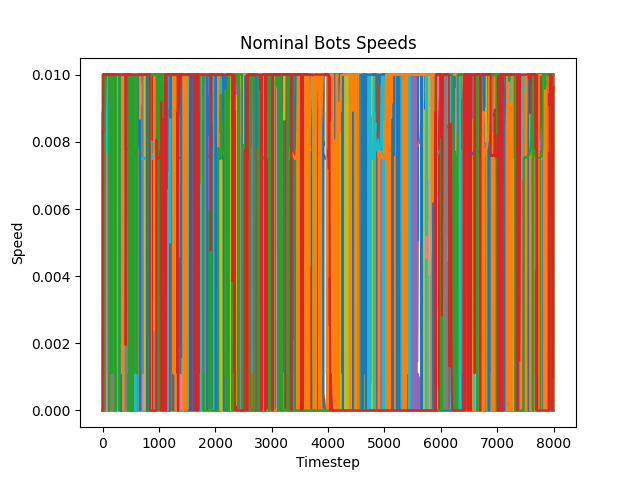
\includegraphics[scale=0.4]{../../Images/Experiments/foraging_size6x8_bot_number38_fault_10_percent_rotating_fault_after_1000/Nominal_Bots_Speeds.png}
					}
					\quad
					\subfloat[Foraging faulty agents speed feature values.\label{fig:foraging_faulty_speed_feature}]{
						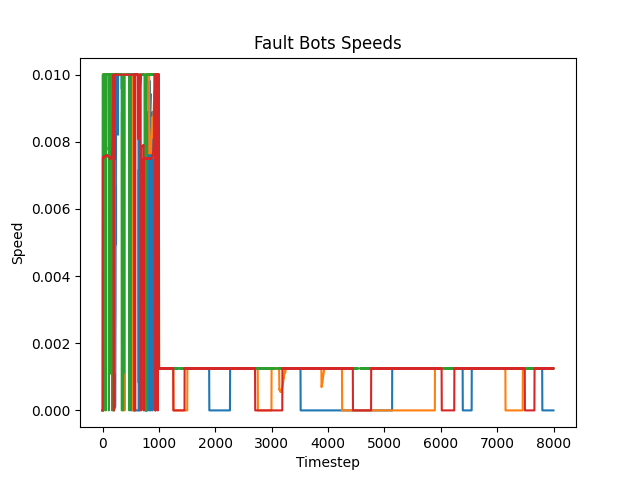
\includegraphics[scale=0.4]{../../Images/Experiments/foraging_size6x8_bot_number38_fault_10_percent_rotating_fault_after_1000/Fault_Bots_Speeds.png}
					}
					\caption{Foraging speed feature values.}
					\label{fig:foraging_speed}
				\end{figure}
			
			\subsubsection{Cumulative Speed}
				This feature has identical characteristics to the speed feature and it is possible to distinguish the faulty robot at first sight (Figure \ref{fig:Foraging_cumulative_speed}). The \verb|time-window| parameter is set to $10$ and the features values show the correlation between the two features.
				\begin{figure}
					\centering
					\subfloat[Foraging nominal agents cumulative speed feature values.
						\label{fig:foraging_nominal_cumulative_speed_feature}]{
						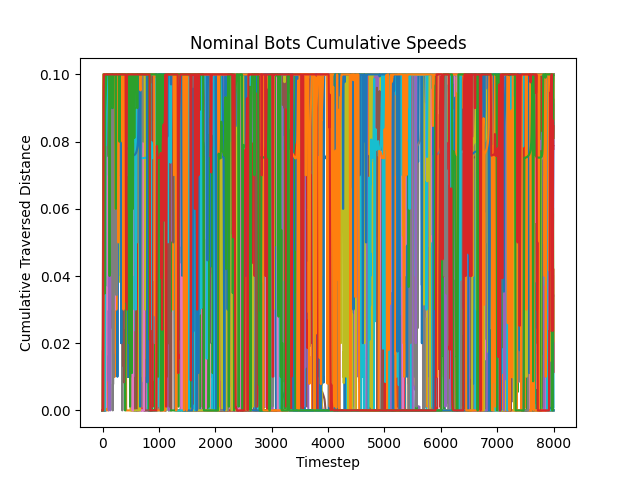
\includegraphics[scale=0.4]{../../Images/Experiments/foraging_size6x8_bot_number38_fault_10_percent_rotating_fault_after_1000/Nominal_Bots_Cumulative_Speeds.png}
					}
					\quad
					\subfloat[Foraging faulty agents cumulative speed feature values.\label{fig:foraging_faulty_cumulative_speed_feature}]{
						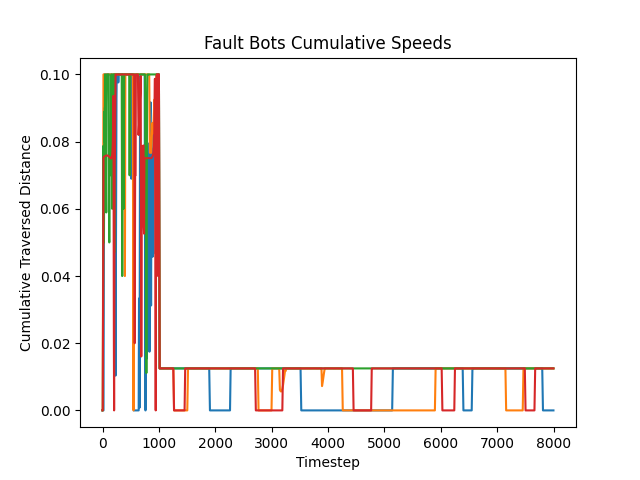
\includegraphics[scale=0.4]{../../Images/Experiments/foraging_size6x8_bot_number38_fault_10_percent_rotating_fault_after_1000/Fault_Bots_Cumulative_Speeds.png}
					}
					\caption{Foraging cumulative speed feature values.}
					\label{fig:Foraging_cumulative_speed}
				\end{figure}
			
			\subsubsection{Neighbors Number}
				The neighbors number feature is not very interesting for the foraging task since the agents spend most of the time wandering around. In Figure \ref{fig:Foraging_neighbors_number} we can see that the faulty agents have similar values with respect to the nominal agents. \\
				In this situation the neighborhood radius value has been set to 2 $m$. This value has to be fine tuned in order to have significant results.
				\begin{figure}
					\centering
					\subfloat[Foraging nominal agents neighbors number feature values.
						\label{fig:foraging_nominal_neighbors_number_feature}]{
						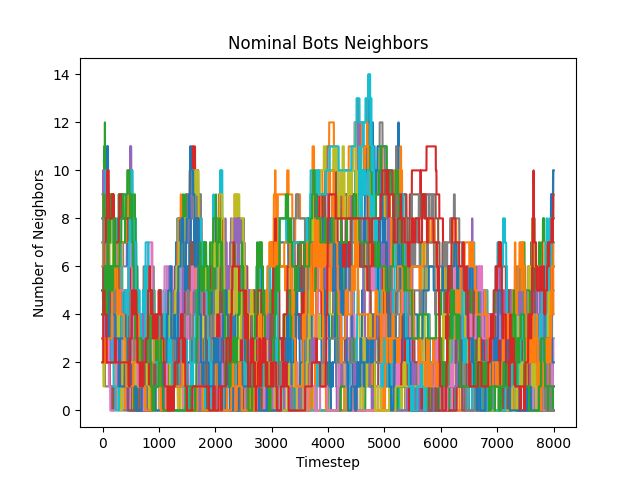
\includegraphics[scale=0.4]{../../Images/Experiments/foraging_size6x8_bot_number38_fault_10_percent_rotating_fault_after_1000/Nominal_Bots_Neighbors.png}
					}
					\quad
					\subfloat[Foraging faulty agents neighbors number feature values.\label{fig:foraging_faulty_neighbors_number_feature}]{
						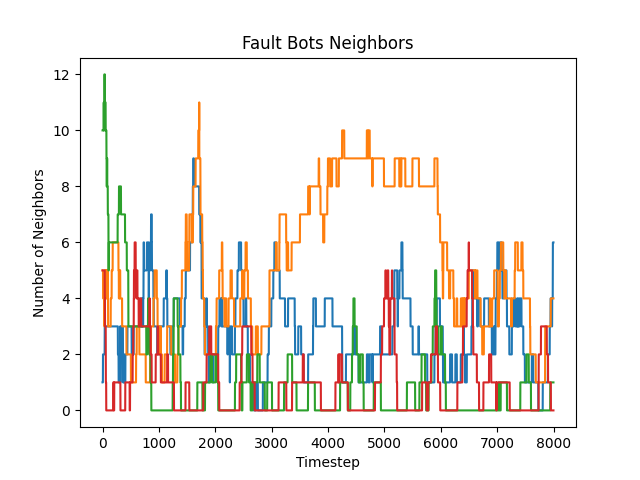
\includegraphics[scale=0.4]{../../Images/Experiments/foraging_size6x8_bot_number38_fault_10_percent_rotating_fault_after_1000/Fault_Bots_Neighbors.png}
					}
					\caption{Foraging neighbors number feature values.}
					\label{fig:Foraging_neighbors_number}
				\end{figure}
			
			\subsubsection{Neighbors Average Distance}
				The neighbors average distance feature highlights information similar to the neighbors number feature with opposite values, in this situation, the high value of the feature denotes a separation of the agent from the swarm. As stated before, this feature does not contain interesting information due to the nature of the task.  In Figure \ref{fig:foraging_neighbors_average_distance} we see that faulty agents and nominal agents have mostly similar values.
				\begin{figure}
					\centering
					\subfloat[Foraging nominal agents neighbors average distance feature values.
						\label{fig:Foraging_nominal_neighbors_average_distance_feature}]{
						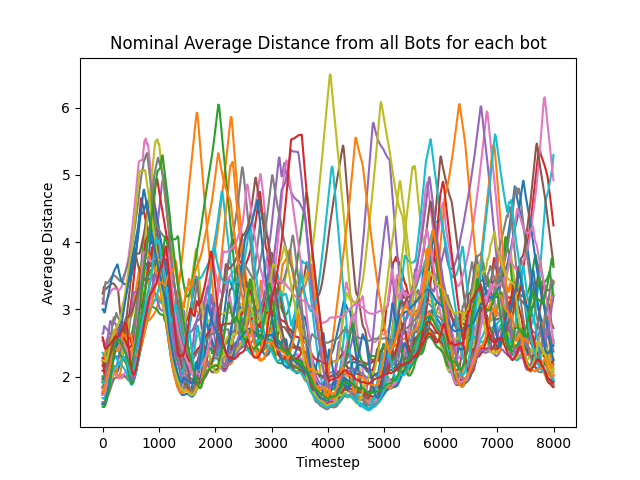
\includegraphics[scale=0.4]{../../Images/Experiments/foraging_size6x8_bot_number38_fault_10_percent_rotating_fault_after_1000/Nominal_Average_Distance_from_all_Bots_for_each_bot.png}
					}
					\quad
					\subfloat[Foraging faulty agents neighbors average distance feature values.\label{fig:foraging_faulty_neighbors_average_distance_feature}]{
						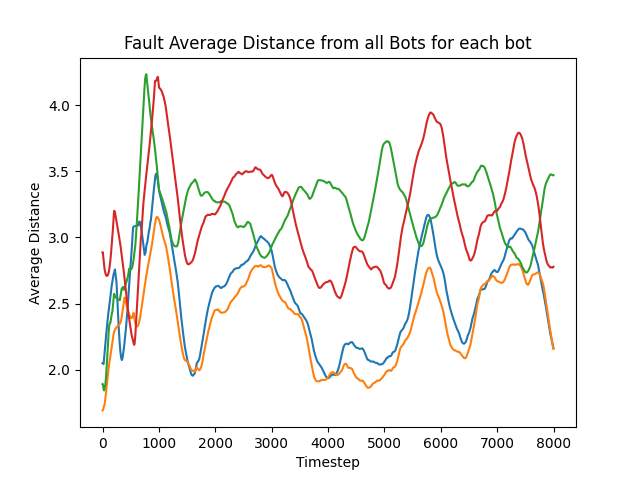
\includegraphics[scale=0.4]{../../Images/Experiments/foraging_size6x8_bot_number38_fault_10_percent_rotating_fault_after_1000/Fault_Average_Distance_from_all_Bots_for_each_bot.png}
					}
					\caption{Foraging neighbors average distance feature values.}
					\label{fig:foraging_neighbors_average_distance}
				\end{figure}
			
			\subsubsection{Centroid Distance}
				From the graphs in Figure \ref{fig:foraging_centroid_distance} we can see that the values have a similar shape to the values shown in Figure \ref{fig:foraging_neighbors_average_distance}, this is because the distance from the centroid can be seen as a mean value of the distance from the other agents.
				\begin{figure}
					\centering
					\subfloat[Foraging nominal agents centroid distance feature values.
						\label{fig:foraging_nominal_centroid_distance_feature}]{
						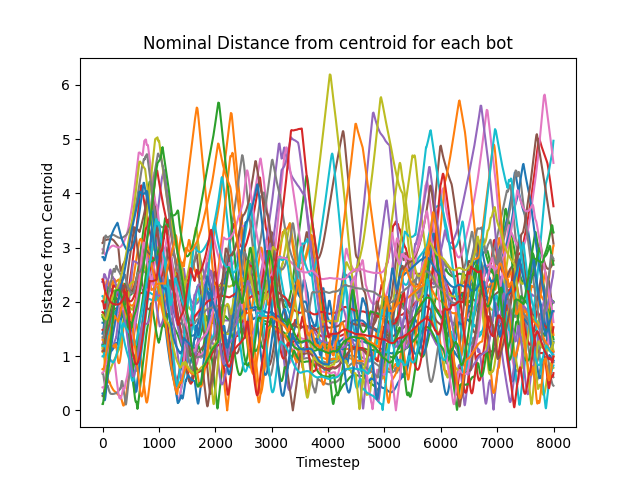
\includegraphics[scale=0.4]{../../Images/Experiments/foraging_size6x8_bot_number38_fault_10_percent_rotating_fault_after_1000/Nominal_Distance_from_centroid_for_each_bot.png}
					}
					\quad
					\subfloat[Foraging faulty agents centroid distance feature values.\label{fig:foraging_faulty_centroid_distance_feature}]{
						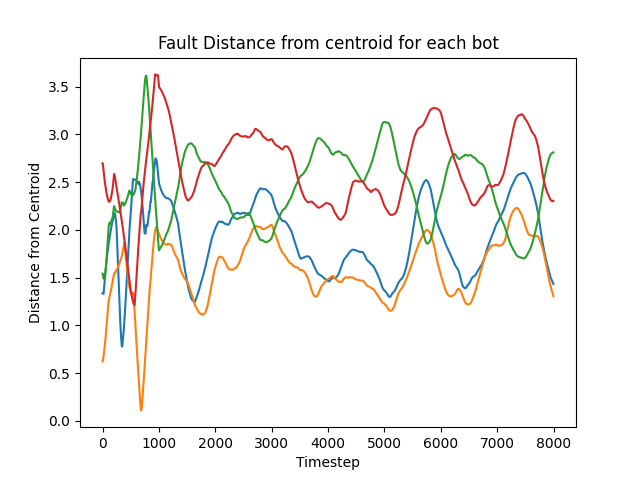
\includegraphics[scale=0.4]{../../Images/Experiments/foraging_size6x8_bot_number38_fault_10_percent_rotating_fault_after_1000/Fault_Distance_from_centroid_for_each_bot.png}
					}
					\caption{Foraging centroid distance feature values.}
					\label{fig:foraging_centroid_distance}
				\end{figure}
			
			\subsubsection{Cumulative Centroid Distance}
				Similarly to the flocking task, these two feature show high correlation and the values in Figure \ref{fig:foraging_cumulative_centroid_distance} depicts the values of Figure \ref{fig:foraging_centroid_distance} multiplied by the \verb|time-window| parameter.
				\begin{figure}
					\centering
					\subfloat[Foraging nominal agents centroid distance feature values.
						\label{fig:foraging_nominal_cumulative_centroid_distance_feature}]{
						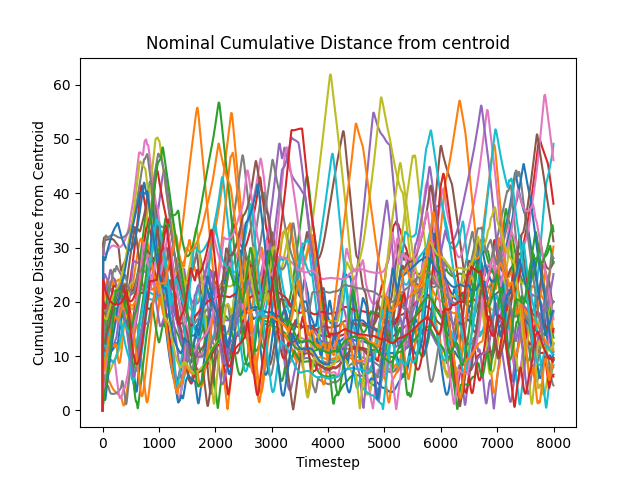
\includegraphics[scale=0.4]{../../Images/Experiments/foraging_size6x8_bot_number38_fault_10_percent_rotating_fault_after_1000/Nominal_Cumulative_Distance_from_centroid.png}
					}
					\quad
					\subfloat[Foraging faulty agents centroid distance feature values.\label{fig:foraging_faulty_cumulative_centroid_distance_feature}]{
						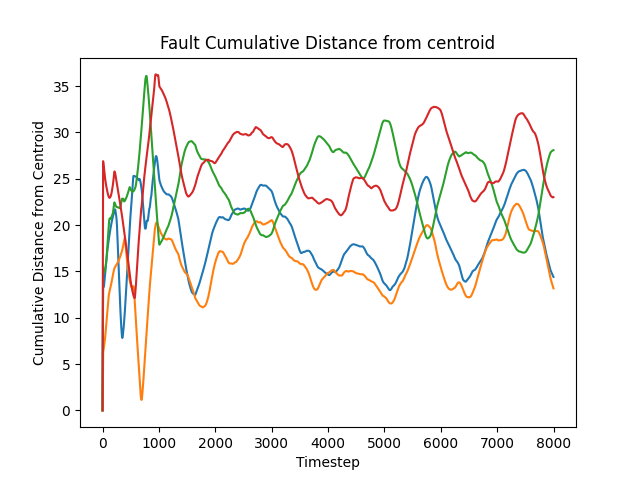
\includegraphics[scale=0.4]{../../Images/Experiments/foraging_size6x8_bot_number38_fault_10_percent_rotating_fault_after_1000/Fault_Cumulative_Distance_from_centroid.png}
					}
					\caption{Foraging centroid distance feature values.}
					\label{fig:foraging_cumulative_centroid_distance}
				\end{figure}
				
			\subsubsection{Position Entropy}
				To analyze this feature we consider a reduced sample of timesteps and a lower number of agents. The graphs shown in Figure \ref{fig:foraging_position_entropy} shows more different values than the graph in Figure \ref{fig:flocking_position_entropy}, however there are not any clearly discriminant characteristic on the graphs that allows us to distinguish nominal agents from faulty agents. As stated before, the values of this feature depend on the tuning of the \verb|time-window| parameter. 
				\begin{figure}
					\centering
					\subfloat[Foraging nominal agents position entropy feature values.
						\label{fig:foraging_nominal_position_entropy_feature}]{
						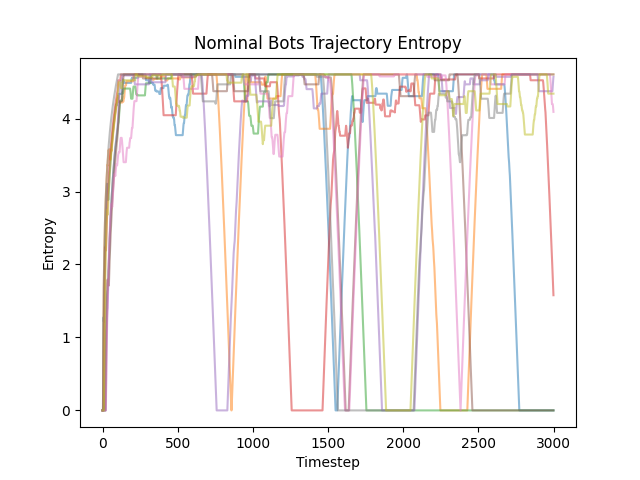
\includegraphics[scale=0.4]{../../Images/Experiments/foraging_size6x8_bot_number38_fault_10_percent_rotating_fault_after_1000/Nominal_Bots_Trajectory_Entropy.png}
					}
					\quad
					\subfloat[Foraging faulty agents position entropy feature values.\label{fig:foraging_faulty_position_entropy_feature}]{
						\includegraphics[scale=0.4]{../../Images/Experiments/foraging_size6x8_bot_number38_fault_10_percent_rotating_fault_after_1000/Fault_Bots_Trajectory_Entropy.png}
					}
					\caption{Foraging position entropy feature values.}
					\label{fig:foraging_position_entropy}
				\end{figure}
			
			\subsubsection{Area Coverage}
				The area coverage feature is identically organized as the flocking task. In Figure \ref{fig:foraging_nominal_agents_area_coverage} we can see that the maximum value reached by the feature decreases with the increase of the area subdivisions, this is because, with the increase of the definition in area partitioning, some areas are too small to be covered by any agent.\\
				The most important difference between nominal (Figure \ref{fig:foraging_nominal_agents_area_coverage}) and faulty agents (Figure \ref{fig:foraging_faulty agents_area_coverage}) is that the faulty agents feature reaches lower values than the nominal agents and it does not increase after the fault is injected. 
				\begin{figure}[H]
					\centering
					\subfloat[4 subdivisions.
						\label{fig:foraging_nominal_4_subdivisions_area_coverage_feature}]{
						\includegraphics[scale=0.22]{../../Images/Experiments/foraging_size6x8_bot_number38_fault_10_percent_rotating_fault_after_1000/Nominal_Single_Bot_Area_Coverage_with_4_subdivisions.png}
					}
					\thinspace
					\subfloat[16 subdivisions.
						\label{fig:foraging_nominal_16_subdivisions_area_coverage_feature}]{
						\includegraphics[scale=0.22]{../../Images/Experiments/foraging_size6x8_bot_number38_fault_10_percent_rotating_fault_after_1000/Nominal_Single_Bot_Area_Coverage_with_16_subdivisions.png}
					}
					\thinspace
					\subfloat[64 subdivisions.
						\label{fig:foraging_nominal_64_subdivisions_area_coverage_feature}]{
						\includegraphics[scale=0.22]{../../Images/Experiments/foraging_size6x8_bot_number38_fault_10_percent_rotating_fault_after_1000/Nominal_Single_Bot_Area_Coverage_with_64_subdivisions.png}
					}
					\thinspace
					\subfloat[256 subdivisions.
						\label{fig:foraging_nominal_256_subdivisions_area_coverage_feature}]{
						\includegraphics[scale=0.22]{../../Images/Experiments/foraging_size6x8_bot_number38_fault_10_percent_rotating_fault_after_1000/Nominal_Single_Bot_Area_Coverage_with_256_subdivisions.png}
					}
					\caption{Foraging nominal agents area coverage feature values.}
					\label{fig:foraging_nominal_agents_area_coverage}
				\end{figure}
			
				\begin{figure}[H]
					\centering
					\subfloat[4 subdivisions.\label{fig:foraging_faulty_4_subdivisions_area_coverage_feature}]{
						\includegraphics[scale=0.22]{../../Images/Experiments/foraging_size6x8_bot_number38_fault_10_percent_rotating_fault_after_1000/Fault_Single_Bot_Area_Coverage_with_4_subdivisions.png}
					}
					\subfloat[16 subdivisions.\label{fig:foraging_faulty_16_subdivisions_area_coverage_feature}]{
						\includegraphics[scale=0.22]{../../Images/Experiments/foraging_size6x8_bot_number38_fault_10_percent_rotating_fault_after_1000/Fault_Single_Bot_Area_Coverage_with_16_subdivisions.png}
					}
					\subfloat[64 subdivisions.\label{fig:foraging_faulty_64_subdivisions_area_coverage_feature}]{
						\includegraphics[scale=0.22]{../../Images/Experiments/foraging_size6x8_bot_number38_fault_10_percent_rotating_fault_after_1000/Fault_Single_Bot_Area_Coverage_with_64_subdivisions.png}
					}
					\subfloat[256 subdivisions.\label{fig:foraging_faulty_256_subdivisions_area_coverage_feature}]{
						\includegraphics[scale=0.22]{../../Images/Experiments/foraging_size6x8_bot_number38_fault_10_percent_rotating_fault_after_1000/Fault_Single_Bot_Area_Coverage_with_256_subdivisions.png}
					}
					\caption{Foraging faulty agents area coverage feature values.}
					\label{fig:foraging_faulty agents_area_coverage}
				\end{figure}
					
			\subsubsection{Area Coverage Speed}
				The graphs are organized like the ones of the area coverage feature. The most distinguishing aspect of this feature is that we can observe the faulty robot that stops exploring earlier than the nominal agents due to the injection of the fault.
				\begin{figure}[H]
					\centering
					\subfloat[4 subdivisions.
						\label{fig:foraging_nominal_4_subdivisions_area_coverage_speed_feature}]{
						\includegraphics[scale=0.22]{../../Images/Experiments/foraging_size6x8_bot_number38_fault_10_percent_rotating_fault_after_1000/Nominal_Single_Bot_Area_Coverage_Speed_with_4_subdivisions.png}
					}
					\thinspace
					\subfloat[16 subdivisions.
						\label{fig:foraging_nominal_16_subdivisions_area_coverage_speed_feature}]{
						\includegraphics[scale=0.22]{../../Images/Experiments/foraging_size6x8_bot_number38_fault_10_percent_rotating_fault_after_1000/Nominal_Single_Bot_Area_Coverage_Speed_with_16_subdivisions.png}
					}
					\thinspace
					\subfloat[64 subdivisions.
						\label{fig:foraging_nominal_64_subdivisions_area_coverage_speed_feature}]{
						\includegraphics[scale=0.22]{../../Images/Experiments/foraging_size6x8_bot_number38_fault_10_percent_rotating_fault_after_1000/Nominal_Single_Bot_Area_Coverage_Speed_with_64_subdivisions.png}
					}
					\thinspace
					\subfloat[256 subdivisions.
						\label{fig:foraging_nominal_256_subdivisions_area_coverage_speed_feature}]{
						\includegraphics[scale=0.22]{../../Images/Experiments/foraging_size6x8_bot_number38_fault_10_percent_rotating_fault_after_1000/Nominal_Single_Bot_Area_Coverage_Speed_with_256_subdivisions.png}
					}
					\caption{Flocking nominal agents area coverage speed feature values.}
					\label{fig:foraging_nominal_agents_area_coverage_speed_feature_values}
				\end{figure}
				
				\begin{figure}[H]
					\centering
					\subfloat[4 subdivisions.\label{fig:foraging_faulty_4_subdivisions_area_coverage_speed_feature}]{
						\includegraphics[scale=0.22]{../../Images/Experiments/foraging_size6x8_bot_number38_fault_10_percent_rotating_fault_after_1000/Fault_Single_Bot_Area_Coverage_Speed_with_4_subdivisions.png}
					}
					\thinspace
					\subfloat[16 subdivisions.\label{fig:foraging_faulty_16_subdivisions_area_coverage_speed_feature}]{
						\includegraphics[scale=0.22]{../../Images/Experiments/foraging_size6x8_bot_number38_fault_10_percent_rotating_fault_after_1000/Fault_Single_Bot_Area_Coverage_Speed_with_16_subdivisions.png}
					}
					\thinspace
					\subfloat[64 subdivisions.\label{fig:foraging_faulty_64_subdivisions_area_coverage_speed_feature}]{
							\includegraphics[scale=0.22]{../../Images/Experiments/foraging_size6x8_bot_number38_fault_10_percent_rotating_fault_after_1000/Fault_Single_Bot_Area_Coverage_Speed_with_64_subdivisions.png}
					}
					\thinspace
					\subfloat[256 subdivisions.\label{fig:foraging_faulty_256_subdivisions_area_coverage_speed_feature}]{
							\includegraphics[scale=0.22]{../../Images/Experiments/foraging_size6x8_bot_number38_fault_10_percent_rotating_fault_after_1000/Fault_Single_Bot_Area_Coverage_Speed_with_256_subdivisions.png}
					}
					\caption{Foraging faulty agents area coverage speed feature values.}
					\label{fig:foraging_faulty_area_coverage_speed}
				\end{figure}
			
			\subsubsection{Global Features}
				\textbf{Swarm Position}\\
				The swarm position feature is the coordinates of the centroid of the swarm. We can see the trajectory followed by the swarm centroid in Figure \ref{fig:flocking_swarm_trajectory} as the bright red line in the middle of the plot among nominal agents (Figure \ref{fig:flocking_nominal_swarm_trajectory}) and faulty agents (Figure \ref{fig:flocking_faulty_swarm_trajectory}).
					\begin{figure}
						\centering
						\subfloat[Swarm trajectory among nominal agents.
							\label{fig:foraging_swarm_trajectory_among_nominal_agents}]{
							\includegraphics[scale=0.3]{../../Images/Experiments/foraging_size6x8_bot_number38_fault_10_percent_rotating_fault_after_1000/Nominal_Bots_Trajectories.png}
						}
						\quad
						\subfloat[Swarm trajectory among faulty agents.\label{fig:foraging_swarm_trajectory_among_faulty_agents}]{
							\includegraphics[scale=0.3]{../../Images/Experiments/foraging_size6x8_bot_number38_fault_10_percent_rotating_fault_after_1000/Fault_Bots_Trajectories.png}
						}
						\label{fig:foraging_swarm_trajectory}
						\caption{Swarm trajectory.}
					\end{figure}
					
					\textbf{Swarm Speed}\\
The swarm speed feature represents the velocity of the swarm centroid. In Figure \ref{fig:foraging_swarm_speed} we can see that the values have a high spike at the beginning, when most of the robots start exploring. Despite this feature showing exactly the fault injection in Figure \ref{fig:flocking_swarm_speed}, in this situation we are unable to observe the fault injection moment due to the nature of the task that does not have a homogeneous behavior.					
					\begin{figure}
						\centering
						\includegraphics[scale=0.4]{../../Images/Experiments/foraging_size6x8_bot_number38_fault_10_percent_rotating_fault_after_1000/Swarm_speed.png}
						\caption{Foraging swarm speed.}
						\label{fig:foraging_swarm_speed}
					\end{figure}
					
			\subsubsection{Swarm Area Coverage}
				The swarm area coverage features illustrate the percentage of area covered by the entirety of the swarm considered each agent. This feature is similar to the area coverage feature seen before in section Area Coverage. As stated above, this is a global feature and does not have the objective to directly identify the fault injection. Nonetheless, the graphs shown in Figure \ref{fig:flocking_swarm_area_coverage_feature_values} do not shown any sign of the presence of the fault injected after 150 $s$.
				\begin{figure}
					\centering
					\subfloat[Foraging swarm 4 subdivisions area coverage feature values.
						\label{fig:foraging_swarm_4_subdivisions_area_coverage_speed_feature}]{
						\includegraphics[scale=0.4]{../../Images/Experiments/foraging_size6x8_bot_number38_fault_10_percent_rotating_fault_after_1000/Swarm_Area_Coverage_with_4_subdivisions.png}
					}
					\quad
					\subfloat[Foraging swarm 16 subdivisions area coverage feature values.\label{fig:flocking_swarm_16_subdivisions_area_coverage_speed_feature}]{
						\includegraphics[scale=0.4]{../../Images/Experiments/foraging_size6x8_bot_number38_fault_10_percent_rotating_fault_after_1000/Swarm_Area_Coverage_with_16_subdivisions.png}
					}
					\quad
					\subfloat[Foraging swarm 64 subdivisions area coverage feature values.
						\label{fig:foraging_swarm_64_subdivisions_area_coverage_speed_feature}]{
						\includegraphics[scale=0.4]{../../Images/Experiments/foraging_size6x8_bot_number38_fault_10_percent_rotating_fault_after_1000/Swarm_Area_Coverage_with_64_subdivisions.png}
					}
					\quad
					\subfloat[Foraging swarm 256 subdivisions area coverage feature values.\label{fig:foraging_swarm_256_subdivisions_area_coverage_feature}]{
						\includegraphics[scale=0.4]{../../Images/Experiments/foraging_size6x8_bot_number38_fault_10_percent_rotating_fault_after_1000/Swarm_Area_Coverage_with_256_subdivisions.png}
					}
					\caption{Foraging swarm area coverage feature values.}
				\end{figure}
					
		\subsection{RMFS Features Analysis}
			The RMFS task of the RAWSim-O simulator is explained in Section \ref{sec:Data_collection:Robot_Mobile_Fulfillment_System}. The robot trajectories can be seen in Figure \ref{fig:RAWSim-O_trajectories}. In this example, we will analyze a simulation of 25 agents with 1 faulty agent. The fault is injected from the beginning of the simulation and the faulty robot travels at 5\% of the maximum speed until the end of the simulation. The positions of all the robots are recorded only when a robot executes its \verb|Act()| function, since this function is not called at every timestep, the time series data points are not evenly distributed in time.
			\subsubsection{Speed}
				As stated before, the speed feature is highly discriminating and we can observe this characteristic in the graph in in Figure \ref{fig:RMFS_speed}.  We can see that the faulty robot does not reach high speeds like nominal robots. 
				\begin{figure}
					\centering
					\subfloat[RMFS nominal agents speed feature values.
						\label{fig:RMFS_nominal_speed_feature}]{
						\includegraphics[scale=0.4]{../../Images/Experiments/warehouse_6x6_10_percent_slowed_at_10fault20211028_17_24/Nominal_Bots_Speeds.png}
					}
					\quad
					\subfloat[RMFS faulty agents speed feature values.\label{fig:RMFS_faulty_speed_feature}]{
						\includegraphics[scale=0.4]{../../Images/Experiments/warehouse_6x6_10_percent_slowed_at_10fault20211028_17_24/Fault_Bots_Speeds.png}
					}
					\caption{RMFS speed feature values.}
					\label{fig:RMFS_speed}
				\end{figure}
			
			\subsubsection{Cumulative Speed}
				From the graphs in Figure \ref{fig:RMFS_cumulative_speed} we can appreciate the same characteristic of the graphs in Figure \ref{fig:RMFS_speed} with fewer spikes and higher values. The speed graphs do not show any discriminating information other than the maximum speed value a robot can reach.
				\begin{figure}
					\centering
					\subfloat[RMFS nominal agents cumulative speed feature values.
						\label{fig:RMFS_nominal_cumulative_speed_feature}]{
						\includegraphics[scale=0.4]{../../Images/Experiments/warehouse_6x6_10_percent_slowed_at_10fault20211028_17_24/Nominal_Bots_Cumulative_Speeds.png}
					}
					\quad
					\subfloat[RMFS faulty agents cumulative speed feature values.\label{fig:RMFS_faulty_cumulative_speed_feature}]{
						\includegraphics[scale=0.4]{../../Images/Experiments/warehouse_6x6_10_percent_slowed_at_10fault20211028_17_24/Fault_Bots_Cumulative_Speeds.png}
					}
					\caption{RMFS cumulative speed feature values.}
					\label{fig:RMFS_cumulative_speed}
				\end{figure}
			
			\subsubsection{Neighbors Number}
				The neighbors number feature (Figure \ref{fig:RMFS_neighbors_number}) does not show any particular difference between nominal robots and faulty robots. Like we have seen in Figure \ref{fig:Foraging_neighbors_number} for the foraging task, the faulty robots have similar values to nominal ones.  The RMFS task does not have the same behavior as the foraging task where robots wander around performing a random walk, in this situation the agents have to follow specific routes and reach specific locations, however, the continuous movements in the warehouse force the robots to visit crowded locations with the same chance of visiting locations with any other robot.\\
				In this situation the neighborhood radius value has been set to 2 $m$. This value has to be fine tuned in order to have significant results.
				\begin{figure}
					\centering
					\subfloat[RMFS nominal agents neighbors number feature values.
						\label{fig:RMFS_nominal_neighbors_number_feature}]{
						\includegraphics[scale=0.4]{../../Images/Experiments/warehouse_6x6_10_percent_slowed_at_10fault20211028_17_24/Nominal_Bots_Neighbors.png}
					}
					\quad
					\subfloat[RMFS faulty agents neighbors number feature values.\label{fig:RMFS_faulty_neighbors_number_feature}]{
						\includegraphics[scale=0.4]{../../Images/Experiments/warehouse_6x6_10_percent_slowed_at_10fault20211028_17_24/Fault_Bots_Neighbors.png}
					}
					\caption{RMFS neighbors number feature values.}
					\label{fig:RMFS_neighbors_number}
				\end{figure}
			
			\subsubsection{Neighbors Average Distance}
				The graphs shown in Figure \ref{fig:RMFS_neighbors_average_distance} have some similarities with the neighbors number feature. Neighbors average distance and the number of neighbors feature are inversely correlated but depict the same behaviors. In Figure \ref{fig:RMFS_faulty_neighbors_average_distance_feature} we can assume that the lowest values are reached when the robot approaches the pick stations. Instead, the higher values depict situations in which the robot is searching for a pod in less visited regions. From the two graphs, we can observe two phases, a first phase in which the feature assumes higher values and a second phase in which the feature assumes on average lower values. This behavior should be analyzed with a complete recording of the simulation, however, we can assume that these values depict a first phase in which the robots visited both pick and replenishment stations, ending in covering a broader area of the warehouse, and a second phase where the robots were closer together may be due to a congestion on the replenishment station or due to an excess of replenishment orders.
				\begin{figure}
					\centering
					\subfloat[RMFS nominal agents neighbors average distance feature values.
						\label{fig:RMFS_nominal_neighbors_average_distance_feature}]{
						\includegraphics[scale=0.4]{../../Images/Experiments/warehouse_6x6_10_percent_slowed_at_10fault20211028_17_24/Nominal_Average_Distance_from_all_Bots_for_each_bot.png}
					}
					\quad
					\subfloat[RMFS faulty agents neighbors average distance feature values.\label{fig:RMFS_faulty_neighbors_average_distance_feature}]{
						\includegraphics[scale=0.4]{../../Images/Experiments/warehouse_6x6_10_percent_slowed_at_10fault20211028_17_24/Fault_Average_Distance_from_all_Bots_for_each_bot.png}
					}
					\caption{RMFS neighbors average distance feature values.}
					\label{fig:RMFS_neighbors_average_distance}
				\end{figure}
			
			\subsubsection{Centroid Distance}
				In Figure \ref{fig:RMFS_centroid_distance} we can observe the same behavior of the neighbors average distance feature shown in Figure \ref{fig:RMFS_neighbors_average_distance}. The only difference we can see between the two features is that the centroid distance shows higher oscillations and less distinguished phases. We could note that the faulty agents have fewer spikes with respect to the nominal agents, we can assume this is a consequence of the lower speeds of faulty robots but it is necessary to implement a model able to interpret time series to exploit these characteristics.
				\begin{figure}
					\centering
					\subfloat[RMFS nominal agents centroid distance feature values.
						\label{fig:RMFS_nominal_centroid_distance_feature}]{
						\includegraphics[scale=0.4]{../../Images/Experiments/warehouse_6x6_10_percent_slowed_at_10fault20211028_17_24/Nominal_Distance_from_centroid_for_each_bot.png}
					}
					\quad
					\subfloat[RMFS faulty agents centroid distance feature values.\label{fig:RMFS_faulty_centroid_distance_feature}]{
						\includegraphics[scale=0.4]{../../Images/Experiments/warehouse_6x6_10_percent_slowed_at_10fault20211028_17_24/Fault_Distance_from_centroid_for_each_bot.png}
					}
					\caption{RMFS centroid distance feature values.}
					\label{fig:RMFS_centroid_distance}
				\end{figure}
				
			\subsubsection{Position Entropy}
				In Figure \ref{fig:RMFS_position_entropy} we analyze a reduced time series with fewer nominal bots to underline the differences between nominal and faulty agents. In particular, we can see that the nominal robots have a higher number of spikes, as stated before this is a consequence of the difference in speed. In Figure \ref{fig:RMFS_position_entropy} we can see that the faulty agent reaches higher values on average than its nominal counterparts. This is an undesired behavior since the slowest robot should visit fewer locations and it should not have high entropy values. However, this feature characteristic is a direct consequence of the \verb|time-window| parameter, confirming once again that each parameter has to be fine tuned for each specific task.
				\begin{figure}
					\centering
					\subfloat[RMFS nominal agents position entropy feature values.
						\label{fig:RMFS_nominal_position_entropy_feature}]{
						\includegraphics[scale=0.4]{../../Images/Experiments/warehouse_6x6_10_percent_slowed_at_10fault20211028_17_24/Nominal_Bots_Trajectory_Entropy.png}
					}
					\quad
					\subfloat[RMFS faulty agents position entropy feature values.\label{fig:RMFS_faulty_position_entropy_feature}]{
						\includegraphics[scale=0.4]{../../Images/Experiments/warehouse_6x6_10_percent_slowed_at_10fault20211028_17_24/Fault_Bots_Trajectory_Entropy.png}
					}
					\caption{RMFS position entropy feature values.}
					\label{fig:RMFS_position_entropy}
				\end{figure}
			
			\subsubsection{Area Coverage}
				The area coverage feature does not depict any new behavior with respect to the graphs analyzed in Figure \ref{fig:flocking_nominal_agents_area_coverage} or Figure \ref{fig:foraging_nominal_agents_area_coverage}. The only clear difference we can appreciate is between Figure \ref{fig:RMFS_nominal_64_subdivisions_area_coverage_feature} and Figure \ref{fig:RMFS_faulty_64_subdivisions_area_coverage_feature} or between  Figure \ref{fig:RMFS_nominal_256_subdivisions_area_coverage_feature} and Figure \ref{fig:RMFS_faulty_256_subdivisions_area_coverage_feature} where the faulty agent reaches lower values on average than the nominal agents.
				\begin{figure}[H]
					\centering
					\subfloat[4 subdivisions.
						\label{fig:RMFS_nominal_4_subdivisions_area_coverage_feature}]{
						\includegraphics[scale=0.22]{../../Images/Experiments/warehouse_6x6_10_percent_slowed_at_10fault20211028_17_24/Nominal_Single_Bot_Area_Coverage_with_4_subdivisions.png}
					}
					\thinspace
					\subfloat[16 subdivisions.
						\label{fig:RMFS_nominal_16_subdivisions_area_coverage_feature}]{
						\includegraphics[scale=0.22]{../../Images/Experiments/warehouse_6x6_10_percent_slowed_at_10fault20211028_17_24/Nominal_Single_Bot_Area_Coverage_with_16_subdivisions.png}
					}
					\thinspace
					\subfloat[64 subdivisions.
						\label{fig:RMFS_nominal_64_subdivisions_area_coverage_feature}]{
						\includegraphics[scale=0.22]{../../Images/Experiments/warehouse_6x6_10_percent_slowed_at_10fault20211028_17_24/Nominal_Single_Bot_Area_Coverage_with_64_subdivisions.png}
					}
					\thinspace
					\subfloat[256 subdivisions.
						\label{fig:RMFS_nominal_256_subdivisions_area_coverage_feature}]{
						\includegraphics[scale=0.22]{../../Images/Experiments/warehouse_6x6_10_percent_slowed_at_10fault20211028_17_24/Nominal_Single_Bot_Area_Coverage_with_256_subdivisions.png}
					}
					\caption{RMFS nominal agents area coverage feature values.}
					\label{fig:RMFS_nominal_agents_area_coverage}
				\end{figure}
			
				\begin{figure}[H]
					\centering
					\subfloat[4 subdivisions.\label{fig:RMFS_faulty_4_subdivisions_area_coverage_feature}]{
						\includegraphics[scale=0.22]{../../Images/Experiments/warehouse_6x6_10_percent_slowed_at_10fault20211028_17_24/Fault_Single_Bot_Area_Coverage_with_4_subdivisions.png}
					}
					\subfloat[16 subdivisions.\label{fig:RMFS_faulty_16_subdivisions_area_coverage_feature}]{
						\includegraphics[scale=0.22]{../../Images/Experiments/warehouse_6x6_10_percent_slowed_at_10fault20211028_17_24/Fault_Single_Bot_Area_Coverage_with_16_subdivisions.png}
					}
					\subfloat[64 subdivisions.\label{fig:RMFS_faulty_64_subdivisions_area_coverage_feature}]{
						\includegraphics[scale=0.22]{../../Images/Experiments/warehouse_6x6_10_percent_slowed_at_10fault20211028_17_24/Fault_Single_Bot_Area_Coverage_with_64_subdivisions.png}
					}
					\subfloat[256 subdivisions.\label{fig:RMFS_faulty_256_subdivisions_area_coverage_feature}]{
						\includegraphics[scale=0.22]{../../Images/Experiments/warehouse_6x6_10_percent_slowed_at_10fault20211028_17_24/Fault_Single_Bot_Area_Coverage_with_256_subdivisions.png}
					}
					\caption{RMFS faulty agents area coverage feature values.}
					\label{fig:RMFS_faulty_agents_area_coverage}
				\end{figure}
			
			\subsubsection{Global Features}
				
				\textbf{Swarm Position}\\
				The swarm position feature is the coordinates of the centroid of the swarm. We can see the trajectory followed by the swarm centroid in Figure \ref{fig:RMFS_swarm_trajectory} as the bright red line in the middle of the plot among nominal agents (Figure \ref{fig:RMFS_swarm_trajectory_among_nominal_agents}) and faulty agents (Figure \ref{fig:RMFS_swarm_trajectory_among_faulty_agents}). Since the data is not evenly distributed in time and we do not have a continuous representation of the robot movements, the swarm position is presented as a set of points mixed with robots trajectories. In particular, we can see that are two main points aggregations, one closer to the middle of the warehouse and one closer to the pick stations. These positions reflect the situation observed for the neighbors average distance graphs in Figure \ref{fig:RMFS_neighbors_average_distance}.
					\begin{figure}[H]
						\centering
						\subfloat[Swarm trajectory among nominal agents.
							\label{fig:RMFS_swarm_trajectory_among_nominal_agents}]{
							\includegraphics[scale=0.3]{../../Images/Experiments/warehouse_6x6_10_percent_slowed_at_10fault20211028_17_24/Nominal_Bots_Trajectories.png}
						}
						\quad
						\subfloat[Swarm trajectory among faulty agents.\label{fig:RMFS_swarm_trajectory_among_faulty_agents}]{
							\includegraphics[scale=0.3]{../../Images/Experiments/warehouse_6x6_10_percent_slowed_at_10fault20211028_17_24/Fault_Bots_Trajectories.png}
						}
						\caption{RMFS Swarm trajectory.}
						\label{fig:RMFS_swarm_trajectory}
					\end{figure}
			
	\section{Metrics}
		In this section, we will introduce the metrics used to evaluate the model performance and explain how to interpret them. 
		\subsection{Confusion Matrix}
			The distinction between nominal and faulty agents is a classification task that falls into the anomaly detection category. Most of the time, anomaly detection implies the presence of an unbalanced set since it is easy to imagine that the anomalies should be less frequent than the nominal data samples. In this situation, analyzing the model performances solely from the accuracy (Equation \ref{eq:classification_accuracy}) values can be misleading. 
			\begin{equation}
				\text{classification accuracy} = \frac{\text{correct predictions}}{\text{total predictions}}
				\label{eq:classification_accuracy}
			\end{equation}
			If we imagine a dataset with very few samples belonging to the faulty class, a trivial model that predicts only the nominal class should obtain high accuracy performance even though it is not rightfully classifying the faulty data samples. To overcome this difficulty we use the confusion matrix which highlights the number of samples classified correctly for each class.  The goal of the confusion matrix is to show how confused is our model while making predictions on the test dataset. The confusion matrix used in our experiments is organized with the actual class instances in the rows and the predicted class instances in the columns, we consider faulty agents for the positive class and negative agents for the negative class. We can see an example of the confusion matrix structure in Table \ref{tab:confusion_matrix_structure}. More precisely, we can see each cell in the matrix as:
			\begin{itemize}
				\item \textbf{True positive:} correctly predicted event values.
				\item \textbf{False positive:} incorrectly predicted event values.
				\item \textbf{True negative:} for correctly predicted no-event values.
				\item \textbf{False negative:} for incorrectly predicted no-event values.
			\end{itemize}
			In particular, a good performance indicator would be to have the majority of the classified samples on the diagonal of the matrix, namely in the true negative and true positive regions.\\
			Furthermore, to extract more information from the confusion matrix, we compute the recall, precision, and f1-score indexes. The precision is defined as:
			\[
				\text{Precision} = \frac{\text{True Positives}}{\text{True Positive} + \text{False Positives}}.
			\]
			This measure is used to “evaluate the fraction of correct classified instances among the ones classified as positive” \cite[pg.52]{Fernandez2018}. The precision values range from $0.0$ to $1.0$ with $0.0$ denoting precision absence and $1.0$ denoting perfect precision.\\
			The recall is defined as:
			\[
				\text{Recall} = \frac{\text{True Positives}}{\text{True Positive} + \text{False Negatives}}
			\]
			and it quantifies the number of correct positive predictions retrieved from all the positive predictions that are possible. The recall values range from $0.0$ to $1.0$ and have the same behavior of precision values.\\
			The use of these two metrics depends on what is the objective of the classifier, if the classifier has to minimize the number of false positives, then it must have high precision, if the classifier has to minimize the number of false negatives, then it must have a high recall.\\
			In order to combine the precision and recall measure, we compute the F1-score. This metric is the harmonic mean of precision and recall and it is computed with the following formula:
			\[
				\text{F1-score} = \frac{2 \cdot \text{Precision} \cdot \text{Recall}}{\text{Precision} + \text{Recall}}.
			\]
			The F1-score can assume values from $0.0$ to $1.0$ and, like all the previous measures, $0.0$ identifies poor performances while $1.0$ identifies perfect performances.
			\renewcommand\arraystretch{1.5}
			\setlength\tabcolsep{0pt}
			\begin{table}
				\centering
					\begin{tabular}{c >{\bfseries}r @{\hspace{0.7em}}c @{\hspace{0.4em}}c @{\hspace{0.7em}}l}
					\multirow{4}{*}{\parbox{1.5cm}{\bfseries\raggedright True\\ Label}} 
					& n$'$ & \MyBox{True}{Negative} & \MyBox{False}{Positive} & \\[2.4em]
					& p$'$ & \MyBox{False}{Negative} & \MyBox{True}{Positive} & \\
					& & \bfseries n & \bfseries p & \\
					& & \multicolumn{2}{c}{\bfseries Predicted Label} \\
				\end{tabular}
				\caption{Confusion matrix structure.}
				\label{tab:confusion_matrix_structure}
			\end{table}
			
		\subsection{Precision Recall Curve}
			In classification tasks, it is useful to measure how the performances change when using different thresholds to distinguish a sample between positive and negative classes.  In binary classification, we can imagine the threshold as the numeric boundary that draws a line between the negative and positive classes. The receiver operating characteristic (ROC) curve and the precision recall curve are two useful metrics to evaluate the classification performance of a model when using different thresholds. In this section, we will explain how the precision-recall curve works and how it can be interpreted. \\
			We have to underline that precision and recall are not directly correlated. If we try to increase the precision of a model by lowering the threshold to identify more positive events, this does not imply that the number of false negatives will decrease so that the recall will increase.\\
			The precision recall curve graphs will also indicate the average precision (AP) measure. The average precision is defined as follows:
			\[
				AP = \sum\limits_{n} (R_n - R_{n-1}) P_n
			\]
			where $P_n$ and $R_n$ are the precision and recall at the $n$-th threshold. This measure identifies the area subtended by the precision recall curve. The AP will range from $0.0$ to $1.0$, values lower than $0.5$ usually mean that the model is performing worse than a random guesser or a trivial model predicting only one class, values higher than $0.5$ mean that the model is able to classify and distinguish a fair amount of samples.  A model with perfect performances will have an AP value around $1.0$ while a model with values around $0.0$ usually presents some errors in the parameters or is trying to classify corrupted data.
	\section{Gradient Boosting Performance Evaluation}
	\label{sec:Experiments:gradient_boosting_performance_evaluation}%
		In this section, we will analyze the performance of our model on the fault detection for the 3 different tasks introduced in Section \ref{sec:running_examples}.  The performances are divided into 3 different sets of features,  these sets aim at collecting different points of view. Even though the goal of our work is to perform fault detection from an external point of view, it is useful to analyze different sets in order to understand which effects and consequences they could have in other approaches. \\
		The first set represents the point of view of the single agent, in this set we have included the following features: position, speed, direction, cumulative speed, position entropy, area coverage, and area coverage speed.\\
		The second set represents the point of view of the single with the acknowledgment of being surrounded by other robots. This feature set includes the following features: position, speed, direction, cumulative speed, neighbors number, neighbors average distance, centroid distance, cumulative centroid distance, position entropy, area coverage, and area coverage speed.\\
		The third and last set represents the point of view of the single agent with complete knowledge of its surroundings and the agents of the swarm. This feature set includes the following features: position, speed, direction, cumulative speed, neighbors number, neighbors average distance, centroid distance, cumulative centroid distance, position entropy, area coverage, area coverage speed, swarm centroid positions, swarm speed, and swarm area coverage.\\
		The gradient boosting model is trained with the following settings:
			\begin{itemize}
				\item \verb|loss = “deviance”|: deviance referes to the logistic regression loss function.
				\item \verb|learning_rate = 0.1|: it is the default value and it is needed to shrink the contribution of each tree.
				\item \verb|max_depth = 3|: this parameter defines the maximum depth of the classification trees. Since the gradient boosting method uses a series of simple classifiers we set this parameter to a low value. However, the documentation states that it should be cross-validated and the performances may be influenced by this parameter.
				\item \verb|n_estimators=500|: it is the maximum number of tree estimators that are introduced in the model. The documentation suggests setting this number to high number since the gradient boosting model is very robust against overfitting.
				\item \verb|max_features=“sqrt”|: it is the maximum number of feature to consider when looking for a split, in this situation, our model consider a number of feature that is the square root of the maximum number of features. The documentation says that for classification tasks it is better to consider a smaller subset of features.
				\item \verb|n_iter_no_change = 5|: this parameter is used to define how many steps without improving validation score are needed to stop the training before its termination. This value is needed to perform early stopping, a technique that prevents the model to overfit on the training data.
				\item \verb|tol = 1e-3|: $1\text{e-}3$ represent the scientific notation in python and it is equal to $1 \cdot 10^{-3} = 0.001$. This is the minimum improvement required to detect a change in the validation set performance while performing early stopping. 
			\end{itemize}
		\subsection{Flocking Fault Detection}
		\label{sec:experiments:flocking_fault_detection}%
			The flocking task simulations we will analyze in this section are described in Section \ref{sec:Flocking}. In section \ref{sec:argos_flocking_simulation_parameters}, we have described a summary of the parameters we have used to collect all the simulations used in the dataset. In general, the overall procedure to execute all the simulations is explained in Algorithm \ref{alg:flocking_simulations_script}. It is implied that every time a simulation is executed its log files are automatically collected. Once the simulation labeled positions have been collected, they are processed to build each feature time series. The elaborated data is processed to obtain an unique time series for the train data set and one for the test dataset. 
			\begin{algorithm}
	 		 	\caption{Flocking Simulation Execution.}
	 		 	\label{alg:flocking_simulations_script}
			    	\begin{algorithmic}[1]
			    	\STATE{nominal-repetitions=15.}
			    	\STATE{positions= \{ North, South, East, West \}. }
			    	\FOR{$i=1$ to nominal-repetitions}
			    		\FOR{\textit{position} in positions}
			    			\STATE{execute nominal simulation from \textit{position}.}
				    	\ENDFOR
			    	\ENDFOR
			    	\STATE{faults= \{10\%, 20\%, 33\%\}. }
			    	\STATE{fault-timesteps = \{ 0, 500, 1500, 4000 \}}
			    	\STATE{single-bot-fault-repetitions = 4. }
			    	\FOR{$i=1$ to single-bot-fault-repetitions}
			    		\FOR{\textit{position} in positions}
			    			\FOR{\textit{fault-time} in fault-timesteps}
				    			\STATE{execute single bot fault simulation from \textit{position} with fault injection after \textit{fault-time}.}
					    	\ENDFOR
				    	\ENDFOR
			    	\ENDFOR
			    	\FOR{\textit{fault-percentage} in faults}
			    		\FOR{\textit{position} in positions}
			    			\FOR{\textit{fault-time} in fault-timesteps}
				    			\STATE{execute \textit{fault-percentage} simulation from \textit{position} with fault injection after \textit{fault-time}.}
					    	\ENDFOR
				    	\ENDFOR
			    	\ENDFOR
			    	\end{algorithmic}
			\end{algorithm}
			
			\subsubsection{Confusion Matrix}
				The confusion matrix describes how many samples of each class the model is able to correctly predict. In Figure \ref{fig:flocking_confusion_matrices} we can see that the gradient boosting model has quite perfect perfomances on the flocking task, the majority of the classified samples is on the diagonal of the confusion matrix and the false positive and false negative cells are almost empty. More precisely, in Table \ref{tab:flocking_gboost_perf_values} we can see that the accuracy, precision, and recall metrics have perfect scores and the F1-score never goes below the 99 percent. Based on which behavioral aspect is more important we can focus either on the precision or on the recall metric. For example, if it is more important to detect immediately a faulty agent because it is dangerous to leave it operating, it is better to have a high recall. On the other hand, if the recovery procedure is expensive in term of times or resources, and the task can be completed without the faulty agent, then its better to focus on the precision and not have a lot of false positives. In this situation all the measures are very promising and it is useless to make any considerations about these values. \\
				In Table \ref{tab:flocking_gboost_perf_values} we can see the exact values of the performance metrics for each feature subset, given the high values and the very small differences among them it does not make sense to assess any influence of the different feature sets.
				\begin{table}
					\center
					\setlength\tabcolsep{0.5em}
					\begin{tabular}{|ccccc|}
						\hline
						\rowcolor{bluepoli!40}
						\multicolumn{1}{|c}{\textbf{Feature Set}} &  \textbf{Accuracy} & \textbf{Precision} & \textbf{Recall} & \textbf{F1}\\ 
						\hline
						1 & 0.9995 & 0.999 & 0.9999 & 0.9995 \\
						\hline
						2 & 0.9996 & 0.9991 & 1.0 & 0.9996 \\
						\hline
						3 & 0.9997 & 0.9993 & 1.0 & 0.9997 \\
						\hline
					\end{tabular}
					\caption{Performances of the gradient boosting model on the flocking task.}
					\label{tab:flocking_gboost_perf_values}
				\end{table}
				\begin{figure}
					\centering
					\subfloat[Feature set 1.\label{fig:flocking_confusion_matrix_feature_set_1}]{
						\includegraphics[scale=0.31]{../../Images/Experiments/flocking_images/All_bots_Shuffled_Conf_Matrix_ShuffledGBoost_Downsampl_x20_set1.png}
					}
					\thinspace
					\subfloat[Feature set 2.\label{fig:flocking_confusion_matrix_feature_set_2}]{
						\includegraphics[scale=0.31]{../../Images/Experiments/flocking_images/All_bots_Shuffled_Conf_Matrix_ShuffledGBoost_Downsampl_x20_set2.png}
					}
					\thinspace
					\subfloat[Feature set 3.\label{fig:flocking_confusion_matrix_feature_set_3}]{
							\includegraphics[scale=0.31]{../../Images/Experiments/flocking_images/All_bots_Shuffled_Conf_Matrix_ShuffledGBoost_Downsampl_x20_set3.png}
					}
					\caption{Confusion matrices of the gradient boosting model performances on the flocking task.}
					\label{fig:flocking_confusion_matrices}
				\end{figure}
				
			\subsubsection{Precision Recall Curve}
				In Figure \ref{fig:flocking_precision_recall_curves} we can see the precision recall curves of the different feature subsets.  It is important to underline that the y-axis of all the graphs starts at values above 0.99 and the AP metric does not show values below $1.00$. The values shown in this section reflect a perfect classification performed by the model. The precision recall curve stays at 1.00 values for the precision for the majority of recall values and lowers to values higher than 0.99 for recall values around 0.9. The plots shown in Figure \ref{fig:flocking_precision_recall_curves} describe a model that is able to perfectly distinguish the positive and negative class for every level of the classification threshold. 
				\begin{figure}
					\centering
					\subfloat[Feature set 1.\label{fig:flocking_prec_rec_curve_feature_set_1}]{
						\includegraphics[scale=0.31]{../../Images/Experiments/flocking_images/All_bots_shuffled_Prec_Rec_Curve_ShuffledGBoost_Downsampl20_set1.png}
					}
					\thinspace
					\subfloat[Feature set 2.\label{fig:flocking_prec_rec_curve_feature_set_2}]{
						\includegraphics[scale=0.31]{../../Images/Experiments/flocking_images/All_bots_shuffled_Prec_Rec_Curve_ShuffledGBoost_Downsampl20_set2.png}
					}
					\thinspace
					\subfloat[Feature set 3.\label{fig:flocking_prec_rec_curve_feature_set_3}]{
							\includegraphics[scale=0.31]{../../Images/Experiments/flocking_images/All_bots_shuffled_Prec_Rec_Curve_ShuffledGBoost_Downsampl20_set3.png}
					}
					\caption{Precision recall curves of the gradient boosting model performances on the flocking task.}
					\label{fig:flocking_precision_recall_curves}
				\end{figure}
			
			\subsubsection{Feature Permutation Results}
				The graphs shown in Figure \ref{fig:flocking_feature_permutation} gather the result of the feature permutation results for the flocking task for the different features sets. As anticipated in Section \ref{sec:Experiments:flocking_feature_analysis},  the speed feature is highly discriminating and the cumulative speed is completely correlated with speed. These characteristics are confirmed by the feature permutation results, in Figure \ref{fig:flocking_feature_permutation_feature_set_1} we see clearly that the cumulative speed feature has a significant influence on the prediction results. Immediately after the cumulative speed feature importance we see the speed feature, this feature has a relevant importance in the classification but not as high as the cumulative speed. The importance values reached by these two features are relevant but not fundamental, a feature importance value of 0.14 (Figure \ref{fig:flocking_feature_permutation_feature_set_1}) for the cumulative speed feature means that the accuracy score of the model on the test set would decrease of 0.14 if the cumulative speed feature is randomly shuffled.This values are significant but do not represent the majority of the accuracy score reached by the model, this means that the feature has discriminant characteristics but is not fundamental for the classification task. In order to appreciate more significant results it would be useful to inspect more subsets combination of feature and see how the feature are correlated.
				\begin{figure}
					\centering
					\subfloat[Feature set 1.\label{fig:flocking_feature_permutation_feature_set_1}]{
						\includegraphics[scale=0.31]{../../Images/Experiments/flocking_images/Feature_importances_using_permutation_n_feats_15.png}
					}
					\thinspace
					\subfloat[Feature set 2.\label{fig:flocking_feature_permutation_feature_set_2}]{
						\includegraphics[scale=0.31]{../../Images/Experiments/flocking_images/Feature_importances_using_permutation_n_feats_19.png}
					}
					\thinspace
					\subfloat[Feature set 3.\label{fig:flocking_feature_permutation_feature_set_3}]{
							\includegraphics[scale=0.31]{../../Images/Experiments/flocking_images/Feature_importances_using_permutation_n_feats_26.png}
					}
					\caption{Feature permutation results on the flocking task.}
					\label{fig:flocking_feature_permutation}
				\end{figure}
		\subsection{Foraging Fault Detection}
			The foraging task simulations we will analyze in this section are described in Section \ref{sec:Foraging}. In section \ref{sec:argos_foraging_simulation_parameters}, we have described a summary of the parameters we have used to collect all the simulations used in the dataset. In general, the overall procedure to execute all the simulations is explained in Algorithm \ref{alg:foraging_simulations_script}. It is implied that every time a simulation is executed its log files are automatically collected. Once the simulation labeled positions have been collected, they are processed to build each feature time series. The elaborated data is processed to obtain an unique time series for the train data set and one for the test dataset. 
			\begin{algorithm}
	 		 	\caption{Foraging Simulation Execution.}
	 		 	\label{alg:foraging_simulations_script}
			    	\begin{algorithmic}[1]
			    	\STATE{nominal-repetitions=15.}
			    	\STATE{arena-dimensions= \{ 5, 6, 7, 8 \}. }
			    	\FOR{$i=1$ to nominal-repetitions}
			    		\FOR{$(x,y)$ in arena-dimensions $\times$ arena-dimensions}
			    			\STATE{execute nominal simulation with arena of size $x \times y$.}
				    	\ENDFOR
			    	\ENDFOR
			    	\STATE{faults= \{10\%, 20\%, 33\%\}. }
			    	\STATE{fault-timesteps = \{ 0, 1000, 4000 \}}
			    	\STATE{single-bot-fault-repetitions = 4. }
			    	\FOR{$i=1$ to single-bot-fault-repetitions}
			    		\FOR{$(x,y)$ in arena-dimensions $\times$ arena-dimensions}
			    			\FOR{\textit{fault-time} in fault-timesteps}
				    			\STATE{execute single bot fault simulation with arena of size $x \times y$ with fault injection after \textit{fault-time}.}
					    	\ENDFOR
				    	\ENDFOR
			    	\ENDFOR
			    	\FOR{\textit{fault-percentage} in faults}
			    		\FOR{$(x,y)$ in arena-dimensions $\times$ arena-dimensions}
			    			\FOR{\textit{fault-time} in fault-timesteps}
				    			\STATE{execute \textit{fault-percentage} simulation with arena of size $x \times y$ with fault injection after \textit{fault-time}.}
					    	\ENDFOR
				    	\ENDFOR
			    	\ENDFOR
			    	\end{algorithmic}
			\end{algorithm}
			\subsubsection{Confusion Matrix}
				The confusion matrix graphs shown in Figure \ref{fig:foraging_confusion_matrices} depict very promising results like in the previous section for the flocking task. The confusion matrices have most of the samples on the diagonal and the cells of the false positive and false negative class have very low values. We can appreciate a small difference between the confusion matrix of the feature set 3 (Figure \ref{fig:foraging_confusion_matrix_feature_set_3}) and the other two confusion matrices of feature set 1 and 2 (Figure \ref{fig:foraging_confusion_matrix_feature_set_1} and Figure \ref{fig:foraging_confusion_matrix_feature_set_2}), in particular we can see that the feature set 3 has a lower number of false negative samples and an higher number of false positive samples. A possible exaplnation of this behavior may be that the hyperspace defined by the feature set 3 arranges the samples such that the model ends up in selecting a threshold more keen to detect positive events instead of negative one, however this interpretation requires further analysis and has to be taken with a grain of salt. \\
				In Table \ref{tab:foraging_gboost_perf_values} we can see the exact values of the accuracy, precision, recall, and F1-score metrics. In this situation the differences between each features set are more evident than the ones of the flocking task (Table \ref{tab:flocking_gboost_perf_values}). In particular we can see some small improvements in the F1-score performances with the increase of the feature set size. The performance improvements of the feature set 3 are a consequence of the high values in the recall metric, as observed before in the confusion matrix, the feature set 3 detects an higher number of positive samples thus increasing the recall while lowering the precision. The interpretation of these results depends on where the model has to put more attention. If the detection of positive samples is critical then it should be better to have an high recall. If the presence of false positives is troublesome and not worth the time, then it is better to have an high precision.
				\begin{table}
					\center
					\setlength\tabcolsep{0.5em}
					\begin{tabular}{|ccccc|}
						\hline
						\rowcolor{bluepoli!40}
						\multicolumn{1}{|c}{\textbf{Feature Set}} &  \textbf{Accuracy} & \textbf{Precision} & \textbf{Recall} & \textbf{F1}\\ 
						\hline
						1 & 0.9184 & 0.8852 & 0.9169 & 0.9008 \\
						\hline
						2 & 0.9232 & 0.9012 & 0.9096 & 0.9054 \\
						\hline
						3 & 0.9306 & 0.8912 & 0.9432 & 0.9164 \\
						\hline
					\end{tabular}
					\caption{Performances of the gradient boosting model on the foraging task.}
					\label{tab:foraging_gboost_perf_values}
				\end{table}
				\begin{figure}
					\centering
					\subfloat[Feature set 1.\label{fig:foraging_confusion_matrix_feature_set_1}]{
						\includegraphics[scale=0.31]{../../Images/Experiments/foraging_images/All_bots_Shuffled_Conf_Matrix_ShuffledGBoost_Downsampl_x20_set1.png}
					}
					\thinspace
					\subfloat[Feature set 2.\label{fig:foraging_confusion_matrix_feature_set_2}]{
						\includegraphics[scale=0.31]{../../Images/Experiments/foraging_images/All_bots_Shuffled_Conf_Matrix_ShuffledGBoost_Downsampl_x20_set2.png}
					}
					\thinspace
					\subfloat[Feature set 3.\label{fig:foraging_confusion_matrix_feature_set_3}]{
							\includegraphics[scale=0.31]{../../Images/Experiments/foraging_images/All_bots_Shuffled_Conf_Matrix_ShuffledGBoost_Downsampl_x20_set3.png}
					}
					\caption{Confusion matrices of the gradient boosting model performances on the foraging task.}
					\label{fig:foraging_confusion_matrices}
				\end{figure}
			\subsubsection{Precision Recall Curve}
				The precision recall curve graphs shown in Figure \ref{fig:foraging_precision_recall_curves} depict interesting results and reflect the satisfactory performance shown by the confusion matrices in Figure \ref{fig:foraging_confusion_matrices}. At first sight, the precision recall curves do not shown any particular difference between each feature set. The AP metric is equivalent among all the feature set and the curve have almost the same slopes with similar values.  Since there is very small or none difference at all between the graphs, it is not possible to make any assumption on the influence of the different feature sets.
				\begin{figure}
					\centering
					\subfloat[Feature set 1.\label{fig:foraging_prec_rec_curve_feature_set_1}]{
						\includegraphics[scale=0.31]{../../Images/Experiments/foraging_images/All_bots_shuffled_Prec_Rec_Curve_ShuffledGBoost_Downsampl20_set1.png}
					}
					\thinspace
					\subfloat[Feature set 2.\label{fig:foraging_prec_rec_curve_feature_set_2}]{
						\includegraphics[scale=0.31]{../../Images/Experiments/foraging_images/All_bots_shuffled_Prec_Rec_Curve_ShuffledGBoost_Downsampl20_set2.png}
					}
					\thinspace
					\subfloat[Feature set 3.\label{fig:foraging_prec_rec_curve_feature_set_3}]{
							\includegraphics[scale=0.31]{../../Images/Experiments/foraging_images/All_bots_shuffled_Prec_Rec_Curve_ShuffledGBoost_Downsampl20_set3.png}
					}
					\caption{Precision recall curves of the gradient boosting model performances on the foraging task.}
					\label{fig:foraging_precision_recall_curves}
				\end{figure}
			\subsubsection{Feature Permutation Results}
				The feature permutation results shown in Figure \ref{fig:foraging_feature_permutation} present some interesting details. In general , we can see that the speed and cumulative speed feature show moderate levels of importance like in the previous graphs for the flocking task. This is a consequence of the nature of the fault injected that forces the robot to have a specific speed. We can observe that these graphs show higher importance for the cumulative speed feature rather than the speed feature, this could suggest that it is better to embed past information into an unique feature.The importance values of the speed and cumulative speed feature are relevant but not very significant. As explained in Section \ref{sec:experiments:flocking_fault_detection} in the feature importance analysis for the flocking task, the feature importance values shown in Figure \ref{fig:foraging_feature_permutation} describe the increase or decrease for the accuracy score. The feature importance graphs for the flocking task show importance values of at most 0.14 that are not a major percentage of the the accuracy scores obtained by the model. Although the importance feature values are modest, we can not make any precise assumption on the real importance of these features since there different subset of features to analyze.\\
				Differently from the flocking task, in this situation we can observe that there are some other features that have small but considerable importance values. More in particular: in Figure \ref{fig:foraging_feature_permutation_feature_set_1} the position entropy feature has relevant values for the first time; in Figure \ref{fig:foraging_feature_permutation_feature_set_2} we can see that the position entropy feature has similar values to the ones in Figure \ref{fig:foraging_feature_permutation_feature_set_1}; lastly, in Figure \ref{fig:foraging_feature_permutation_feature_set_3} there is the position entropy feature that has relevant values but it is overcome by the area coverage with 256 subdivisions. The values reached by these features do not have significant influence on the model performances but they definitely have some influence in the classification task and can be further analyzed in more detailed experiments.
				\begin{figure}
					\centering
					\subfloat[Feature set 1.\label{fig:foraging_feature_permutation_feature_set_1}]{
						\includegraphics[scale=0.31]{../../Images/Experiments/foraging_images/Feature_importances_using_permutation_n_feats_15.png}
					}
					\thinspace
					\subfloat[Feature set 2.\label{fig:foraging_feature_permutation_feature_set_2}]{
						\includegraphics[scale=0.31]{../../Images/Experiments/foraging_images/Feature_importances_using_permutation_n_feats_19.png}
					}
					\thinspace
					\subfloat[Feature set 3.\label{fig:foraging_feature_permutation_feature_set_3}]{
							\includegraphics[scale=0.31]{../../Images/Experiments/foraging_images/Feature_importances_using_permutation_n_feats_26.png}
					}
					\caption{Feature permutation results on the foraging task.}
					\label{fig:foraging_feature_permutation}
				\end{figure}
				
		\subsection{RMFS Fault Detection}
			The RMFS task simulations we will analyze in this section are described in Section \ref{sec:Data_collection:Robot_Mobile_Fulfillment_System}. In section \ref{sec:fault_detection:RAWSim-O_fulfillment_system}, we have described a summary of the parameters we have used to collect all the simulations used in the dataset. In general, the overall procedure to execute all the simulations is explained in Algorithm \ref{alg:RMFS_simulations_script}. It is implied that every time a simulation is executed its log files are automatically collected. Once the simulation labeled positions have been collected, they are processed to build each feature time series. The elaborated data is processed to obtain an unique time series for the train data set and one for the test dataset. 
			\begin{algorithm}
	 		 	\caption{RMFS Simulation Execution.}
	 		 	\label{alg:RMFS_simulations_script}
			    	\begin{algorithmic}[1]
			    	\STATE{nominal-repetitions=4.}
			    	\STATE{aisles-numbers = \{ 5, 6, 7, 8 \}. }
			    	\FOR{$i=1$ to nominal-repetitions}
			    		\FOR{$(x,y)$ in aisles-numbers $\times$ aisles-numbers}
			    			\STATE{execute nominal simulation with warehouse of size $x \times y$.}
				    	\ENDFOR
			    	\ENDFOR
			    	\STATE{faults = \{10\%, 20\%, 33\%\}. }
			    	\STATE{fault-timesteps = \{ 0, 1000, 4000 \}}
			    	\STATE{single-bot-fault-repetitions = 4. }
			    	\FOR{$i=1$ to single-bot-fault-repetitions}
			    		\FOR{$(x,y)$ in aisles-numbers $\times$ aisles-numbers}
			    			\FOR{\textit{fault-time} in fault-timesteps}
				    			\STATE{execute single bot fault simulation with warehouse of size $x \times y$ with fault injection after \textit{fault-time}.}
					    	\ENDFOR
				    	\ENDFOR
			    	\ENDFOR
			    	\FOR{\textit{fault-percentage} in faults}
			    		\FOR{$(x,y)$ in arena-dimensions $\times$ arena-dimensions}
			    			\FOR{\textit{fault-time} in fault-timesteps}
				    			\STATE{execute \textit{fault-percentage} simulation with warehouse of size $x \times y$ with fault injection after \textit{fault-time}.}
					    	\ENDFOR
				    	\ENDFOR
			    	\ENDFOR
			    	\end{algorithmic}
			\end{algorithm}
			\subsubsection{Confusion Matrix}
				In Figure \ref{fig:RMFS_confusion_matrices} we can see the confusion matrices of the model performances for the RMFS task. The confusion matrices graphs depict promising performances, in particular, the samples are mostly in the diagonal of the matrix and the false negative and false positive cells have fairly low numbers. From the confusion matrices graphs we can observe there is a mild trend from feature set 1 to feature set 3 on selecting more positive samples.  This trend can be seen on the colors of the predicted positive class column that gets more intense from the left to the right. The bias towards the positive class can also be confirmed in Table \ref{tab:RMFS_gboost_perf_values}, we can see that from feature set 1 to feature set 3 the precision gets lower while the recall improves significantly. 
				\begin{table}
					\center
					\setlength\tabcolsep{0.5em}
					\begin{tabular}{|ccccc|}
						\hline
						\rowcolor{bluepoli!40}
						\multicolumn{1}{|c}{\textbf{Feature Set}} &  \textbf{Accuracy} & \textbf{Precision} & \textbf{Recall} & \textbf{F1}\\ 
						\hline
						1 & 0.885 & 0.9184 & 0.8167 & 0.8646\\
						\hline
						2 & 0.8789 & 0.8671 & 0.8629 & 0.865 \\
						\hline
						3 & 0.8761 & 0.8402 & 0.8946 & 0.8665 \\
						\hline
					\end{tabular}
					\caption{Performances of the gradient boosting model on the RMFS task.}
					\label{tab:RMFS_gboost_perf_values}
				\end{table}
				\begin{figure}
					\centering
					\subfloat[Feature set 1.\label{fig:RMFS_confusion_matrix_feature_set_1}]{
						\includegraphics[scale=0.31]{../../Images/Experiments/warehouse_images/All_bots_Shuffled_Conf_Matrix_ShuffledGBoost_Downsampl_x20_set1.png}
					}
					\thinspace
					\subfloat[Feature set 2.\label{fig:RMFS_confusion_matrix_feature_set_2}]{
						\includegraphics[scale=0.31]{../../Images/Experiments/warehouse_images/All_bots_Shuffled_Conf_Matrix_ShuffledGBoost_Downsampl_x20_set2.png}
					}
					\thinspace
					\subfloat[Feature set 3.\label{fig:RMFS_confusion_matrix_feature_set_3}]{
							\includegraphics[scale=0.31]{../../Images/Experiments/warehouse_images/All_bots_Shuffled_Conf_Matrix_ShuffledGBoost_Downsampl_x20_set3.png}
					}
					\caption{Confusion matrices of the gradient boosting model performances on the RMFS task.}
					\label{fig:RMFS_confusion_matrices}
				\end{figure}
				
			\subsubsection{Precision Recall Curve}
				The precision recall curve graphs shown in Figure \ref{fig:RMFS_precision_recall_curves} reflect the behavior seen in Table \ref{tab:RMFS_gboost_perf_values}. From the left, we can see that the precision recall curve of the feature set 1 has an average precision of 0.95 while the other two graphs have an average precision of 0.96. More in particular, the precision recall curve of feature set 3 has an area under the curve bigger than feature set 2. \\
				From the behaviors of the precision recall curve graphs we can say that the samples mix together in some areas of the hyperspace because the model drops in performance with the modification of the classification threshold. This characteristic can be seen in the decrease of the curve before the small step at the end. 
				\begin{figure}
					\centering
					\subfloat[Feature set 1.\label{fig:RMFS_prec_rec_curve_feature_set_1}]{
						\includegraphics[scale=0.31]{../../Images/Experiments/warehouse_images/All_bots_shuffled_Prec_Rec_Curve_ShuffledGBoost_Downsampl20_set1.png}
					}
					\thinspace
					\subfloat[Feature set 2.\label{fig:RMFS_prec_rec_curve_feature_set_2}]{
						\includegraphics[scale=0.31]{../../Images/Experiments/warehouse_images/All_bots_shuffled_Prec_Rec_Curve_ShuffledGBoost_Downsampl20_set2.png}
					}
					\thinspace
					\subfloat[Feature set 3.\label{fig:RMFS_prec_rec_curve_feature_set_3}]{
							\includegraphics[scale=0.31]{../../Images/Experiments/warehouse_images/All_bots_shuffled_Prec_Rec_Curve_ShuffledGBoost_Downsampl20_set3.png}
					}
					\caption{Precision recall curves of the gradient boosting model performances on the RMFS task.}
					\label{fig:RMFS_precision_recall_curves}
				\end{figure}
			
			\subsubsection{Feature Permutation Results}
				The feature importance graphs shown in Figure \ref{fig:RMFS_feature_permutation} present a new characteristic that did not appear in the previous tasks. The graphs show that the position entropy feature has the highest feature importance value, immediately followed by the speed and cumulative speed features. Since the speed feature and the cumulative speed feature still have modestly high values, we can not say that the position entropy is the most discriminant feature. Considering the small value difference between the feature importance of the speed feature and the position entropy feature on the feature set, this behavior could vanish with a different permutation of the dataset or a new training execution. In order to confirm the importance of the position entropy feature this results should be cross validated with multiple training executions. However, it is interesting to see that the position entropy features presents significant importance values across the three feature sets. This result can be a hint on which features to analyze in the future analysis.\\
				All the other features in the feature sets, other than speed and cumulative speed, have insignificant values and do not show any interesting quality.\\
				In the end, when we perform feature importance using highly correlated features, like speed and cumulative speed for example,  there are some precautions to take. When we compute the feature permutation importance of two correlated features, the model still has access to the correlated feature and the final results will have a lower importance score for the feature under analysis. This underlines that using correlated features should be avoided and when done it has to be taken under consideration for the feature importance scores. \\
				Another aspect that would be interesting to analyze is the difference of the feature importance between the training dataset and the test dataset. This analysis would highlight features that may lead the model to overfit. If a feature is important on the training set but not on the test set, it is likely to drive the model to overfit.
				\begin{figure}
					\centering
					\subfloat[Feature set 1.\label{fig:RMFS_feature_permutation_feature_set_1}]{
						\includegraphics[scale=0.31]{../../Images/Experiments/warehouse_images/Feature_importances_using_permutation_n_feats_15.png}
					}
					\thinspace
					\subfloat[Feature set 2.\label{fig:RMFS_feature_permutation_feature_set_2}]{
						\includegraphics[scale=0.31]{../../Images/Experiments/warehouse_images/Feature_importances_using_permutation_n_feats_19.png}
					}
					\thinspace
					\subfloat[Feature set 3.\label{fig:RMFS_feature_permutation_feature_set_3}]{
							\includegraphics[scale=0.31]{../../Images/Experiments/warehouse_images/Feature_importances_using_permutation_n_feats_26.png}
					}
					\caption{Feature permutation results on the RMFS task.}
					\label{fig:RMFS_feature_permutation}
				\end{figure}
\end{document}
